\documentclass[11pt]{article}
\usepackage[margin=1in]{geometry}
\usepackage{amsmath,amssymb,amsthm}
\usepackage{graphicx}
\usepackage{booktabs}
\usepackage{hyperref}
\usepackage[numbers,sort&compress]{natbib}
\usepackage{xcolor}

\newtheorem{definition}{Definition}
\newtheorem{remark}{Remark}
\newtheorem{proposition}{Proposition}
\newtheorem{corollary}{Corollary}

\title{Random Matrix Theory and Dyson-Brownian-Motion Diagnostics for \\
Breast Cancer Coexpression Networks: A Monte-Carlo-Validated \\
Framework Applied to TCGA-BRCA}

\author{
Julio C\'esar Galindo L\'opez$^{1,*}$ \and Enrique Hern\'andez-Lemus$^{2}$
\\[4pt]
{\small $^{1}$ Facultad de Ciencias Empresariales, Universidad Panamericana, Ciudad de M\'exico}\\
{\small $^{2}$ Computational Systems Biology and Integrative Genomics Laboratory,}\\
{\small Instituto Nacional de Medicina Gen\'omica (INMEGEN)}\\[6pt]
{\small $^{*}$Correspondence: Julio C\'esar Galindo L\'opez, \texttt{jcgalindo@up.edu.mx}}
}

\date{September 2026}

\begin{document}
\maketitle

\begin{abstract}
\noindent\textbf{Background:}
Random matrix theory (RMT) offers a principled way to decide which
correlations in a noisy, finite-sample gene-expression matrix reflect
real biology rather than sampling noise. We combine the classical
RMT correlation-threshold method with a Monte Carlo permutation null,
a Dyson-Brownian-motion repulsion diagnostic, spectral
entropy, and a graph-theoretic comparison against random-graph nulls,
and apply the full pipeline to real bulk RNA-seq data from The Cancer
Genome Atlas breast cancer cohort (TCGA-BRCA), comparing two
clinically defined, non-overlapping cohorts: triple-negative breast
cancer (TNBC, $n=119$) and luminal A (LumA, $n=430$), 1500 genes
selected by variance across all 1218 samples, cohort-blind.

\noindent\textbf{Results:}
The RMT threshold method selects $\tau^*=0.45$ for TNBC and
$\tau^*=0.25$ for LumA; the gap survives a matched-sample-size check
and a Monte Carlo permutation null, which shows both thresholds lie
well beyond what dense-matrix universality alone could produce. Fewer
than $2\%$ of candidate genes' correlation directions exceed the
Marchenko--Pastur noise bulk yet capture roughly half the total
variance per cohort, and the leading such directions are thematically
coherent multi-gene programs (collagen/ECM, interferon, keratin)
rather than single-gene artifacts. Tracking the top eigenvalues as the
TNBC sample grows one patient at a time shows several pairs undergoing
Dyson-type level repulsion (approach, then reopen, rather than cross).
A wavelet multiscale decomposition failed a random-ordering control on
real data but a synthetic positive control shows it works correctly at
both scales given sufficient signal --- the real-data failure was a
weak-ordering-axis problem, not a method problem. A classifier
distinguishing TNBC from LumA reaches $\approx\!98\%$ accuracy
regardless of feature-selection method, including random gene sets; a
genetic-algorithm search finds a modest, real improvement ($99.45\%$)
without breaking the ceiling. Tracking that same classifier's own
weight-matrix eigenvalues across SGD training (the model-side half of
the Dyson-repulsion question) finds far less reliable repulsion than on
the data side over a full training run, but what repulsion is present
concentrates almost entirely in the pre-convergence transient, a
12-fold difference against the post-convergence window. Applying the
identical RMT machinery to real single-cell RNA-seq data for the first
time in this program (GSE176078, one TNBC patient, 7986 cells) finds a
real, permutation-confirmed threshold in a regime where the gene-to-cell
ratio inverts relative to the bulk cohorts; the largest spiked
eigenvalues split cleanly into real cell-type axes (immune, myeloid,
epithelial, matching independent cell-type annotation) and known
single-cell technical artifacts (ribosomal content, dissociation
stress), a distinction the bulk analysis never had to draw.

\noindent\textbf{Conclusions:}
Combining a static RMT threshold with an explicit Monte Carlo null and
a Dyson-repulsion diagnostic surfaces real, validated structure in
TCGA-BRCA coexpression networks and in single-cell data alike, and the
same discipline exposes three honest negative results (the wavelet
real-data application, the classification benchmark's ceiling effect,
and the classifier's weight-matrix repulsion outside its training
transient) rather than dropping them.
All numbers are produced by included, re-runnable code; one originally
proposed line remains genuinely unattempted with real data (3D genomic
structure via Hi-C), stated as such with a concretely-sized next step.
\end{abstract}

\noindent\textbf{Keywords:} random matrix theory; gene coexpression networks;
triple-negative breast cancer; TCGA; Monte Carlo permutation test;
Dyson Brownian motion; Marchenko--Pastur law

\section{Background}

Triple-negative breast cancer (TNBC) --- tumors negative for estrogen
receptor, progesterone receptor, and HER2 --- lacks the targeted
therapies available for hormone-receptor-positive or HER2-enriched
disease, and remains transcriptionally and clinically heterogeneous
\citep{foulkes2010}. Network-based approaches that treat gene
coexpression as a graph, rather than testing genes one at a time, have
become a standard tool for finding this heterogeneity's structure,
and the Hern\'andez-Lemus group has applied several such approaches
directly to breast cancer: multilayer information-theoretic
transcriptional networks \citep{multilayer2021}, $k$-core structural
analysis \citep{kcore2021}, and multi-omic subtype-specific interaction
networks \citep{multiomic2022}. The group's own network-inference
pipeline for breast cancer, publicly available as the CSB-IG
\texttt{breast\_cancer\_networks} and \texttt{parallel-aracne}
repositories, is built on ARACNE \citep{margolin2006}: mutual
information between every gene pair, pruned by the Data Processing
Inequality, with a bootstrap procedure (the NIMEA pipeline,
\texttt{CSB-IG/BioNetworkInference\_ModularAnalysis}) used to set the
mutual-information significance threshold and Infomap used for module
detection --- an information-theoretic route to the same underlying
question this paper asks with a spectral one: given a noisy,
finite-sample gene-expression matrix, which pairwise associations are
real? The RMT threshold in Sec.~\ref{sec:tau-sweep} and the
group's own bootstrap-calibrated mutual-information threshold are two
different statistical routes to a threshold-selection problem neither
one has an obviously superior claim to; running both on the same TNBC
cohort and comparing the resulting hub genes and modules is a direct,
concrete extension of this paper, using tooling the group already has
in production rather than anything new.

A separate line of work asks a narrower but sharper question: given a
correlation matrix built from noisy, finite-sample gene-expression
data, which correlations reflect real biological structure and which
are sampling noise? Random matrix theory answers this by comparing the
empirical eigenvalue spectrum against the null spectrum expected from a
random (structureless) matrix of the same size. \citet{luo2007}
formalized this into a concrete recipe for gene coexpression networks:
sweep a correlation threshold $\tau$, and select the value at which the
nearest-neighbor eigenvalue spacing distribution switches from Poisson
(uncorrelated, structureless) to the Gaussian-orthogonal-ensemble (GOE)
Wigner surmise (correlated, structured) --- a transition driven by
level repulsion, the same mechanism Wigner and Dyson identified in
nuclear spectra and later in general Hermitian random matrices
\citep{dyson1962}. The method has since been used at genome scale
\citep{gao2012} and specifically in cancer gene networks
\citep{cancer2018}.

Two further questions motivate the present paper. First, is the
selected threshold real, or an artifact of the asymptotic
Marchenko--Pastur/Wigner-surmise null used to select it? A Monte Carlo
permutation null --- shuffling each gene's values across patients
independently, destroying every real correlation while keeping each
gene's own marginal distribution fixed, the same kind of null the
group's own NIMEA pipeline uses to calibrate its mutual-information
threshold (Sec.~\ref{sec:montecarlo}, below) --- answers this directly
rather than relying on asymptotics alone. Second, \citet{aarts2024}
showed that the weight matrices of a neural network undergoing
stochastic-gradient-descent training evolve according to Dyson's
(1962) eigenvalue Brownian motion, with the same level-repulsion
mechanism at work --- suggesting that the repulsion diagnostic itself,
not just the static threshold it eventually selects, carries
information, and that it applies equally to a biological correlation
matrix and to the training dynamics of a classifier built on top of it.

This paper does three things. It states, as a single explicit
framework, how a static RMT threshold, a Monte Carlo permutation null,
and a Dyson-repulsion diagnostic relate to one another (Methods). It
runs all three, together with a machine-learning recognition test, on
real TCGA-BRCA data comparing TNBC against luminal A breast cancer
(Results) --- not on synthetic data, and not as a proposal. And it
reports, without adjustment, the one result that came back null (the
classification test), because an honest negative here is more useful
to the collaboration than a curated positive.

\subsection{Mathematical background}
\label{sec:math}

We collect here, precisely, the four pieces of random matrix theory the
rest of the paper uses, since each plays a distinct role and the
distinctions matter for how the results should be read.

\begin{definition}[Wigner ensemble and the GOE]
\label{def:goe}
A Gaussian orthogonal ensemble (GOE) matrix is a real symmetric
$N\times N$ matrix $H$ with $H_{ii}\sim\mathcal N(0,2)$ and
$H_{ij}=H_{ji}\sim\mathcal N(0,1)$ ($i<j$) independently. As
$N\to\infty$, its empirical eigenvalue distribution (after rescaling)
converges to Wigner's semicircle law, and, crucially for us, the
distribution of \emph{spacings} between adjacent eigenvalues, after
unfolding to unit mean spacing, converges to the Wigner surmise
$p(s)=\frac{\pi}{2}s\,e^{-\pi s^2/4}$ --- the density used throughout
this paper as the ``correlated/structured'' null.
\end{definition}

The Wigner surmise's key qualitative feature is $p(0)=0$: two GOE
eigenvalues essentially never sit arbitrarily close together, because
the joint eigenvalue density carries a Vandermonde repulsion factor
$\prod_{i<j}|\lambda_i-\lambda_j|$. This is the same repulsion term that
appears, dynamically rather than statically, in Dyson's model below;
the static NNSD test and the dynamic trajectory test in
Sec.~\ref{sec:results-dyson} are two different windows onto the same
underlying mechanism, not two unrelated diagnostics. By contrast, a
matrix with no such structure (e.g.\ a diagonal matrix of i.i.d.\
values, or --- the case relevant here --- a correlation matrix
thresholded so sparsely that it behaves like a disconnected random
graph) has independent eigenvalues and Poisson-distributed spacings
$p(s)=e^{-s}$, which \emph{does} allow near-degeneracies
($p(0)=1$, maximal at zero spacing). The Luo et al.\ method
\citep{luo2007} used throughout Sec.~\ref{sec:tau-sweep} operationalizes
exactly this contrast: sparse/uninformative thresholds look Poisson,
and the threshold at which the spectrum first looks GOE-like is read as
the point where real correlation structure first dominates chance.

\begin{remark}[The $N\to\infty$ limit, free probability, and Hilbert spaces]
The Wigner semicircle law referenced above is a statement about
$N\times N$ GOE matrices as $N\to\infty$: the empirical spectral
measure converges to a fixed limiting shape. Free probability theory
\citep{voiculescu1991} recasts this convergence operator-theoretically:
a sequence of independent GOE (or Wigner) matrices converges, in the
sense of joint moments, to a family of \emph{free} self-adjoint
elements in a von Neumann algebra equipped with a trace --- a
noncommutative probability space built on a Hilbert space, in exactly
the sense operator algebras use the term. In that limit the semicircle
law is not an analogy to the Gaussian but its literal free-probabilistic
counterpart: it is the fixed point of free convolution the way the
Gaussian is the fixed point of classical convolution (the free Central
Limit Theorem), and ``freeness'' is the operator-algebraic
substitute for classical independence that makes this work. None of
this machinery is invoked computationally in this paper --- every
matrix here is finite ($p=1500$ or $60$), and every claim is checked
directly on that finite matrix or by finite-$n$ Monte Carlo, never by
appeal to the $N\to\infty$ operator-algebraic limit --- but it is the
reason the semicircle/GOE machinery generalizes so far beyond Gaussian
random matrices in the first place: free probability, not Gaussianity,
is the real source of the universality being leaned on throughout
Sec.~\ref{sec:tau-sweep} and Sec.~\ref{sec:montecarlo}. A standard
modern reference for this whole circle of ideas, including the
Dyson Brownian motion and Tracy--Widom material below, is
\citet{aguz2010}. Ben~Arous and Guionnet sharpened the convergence
itself into a large deviations principle \citep{benarousguionnet1997}:
the empirical spectral measure of a GOE matrix does not merely converge
to the semicircle law, it does so with an exponentially small
probability of any other outcome, governed by a rate function built
from Voiculescu's free (non-commutative) entropy --- the same notion
of entropy invoked, in the unrelated but same-named finite-matrix
sense, by the spectral entropy diagnostic of
Sec.~\ref{sec:entropy}. The two entropies are different
objects (one a large-deviations rate functional on the space of
limiting measures, the other a Shannon entropy of one finite matrix's
own normalized spectrum) and this paper does not conflate them; they
share a name, and a spectral origin, for a real reason worth
recording rather than treating as coincidence.
\end{remark}

\begin{remark}[Four-moment universality: why finite, non-Gaussian data is not a problem]
The free-probability remark above addresses the $N\to\infty$ limit;
a sharper, finite-$N$ statement addresses the objection that TCGA-BRCA
expression data is not Gaussian at all. \citet{taovu2011} proved a
Four Moment Theorem: local eigenvalue statistics of a Wigner
matrix (spacing distributions, correlation functions, and in
particular the GOE/Wigner-surmise statistics used throughout
Sec.~\ref{sec:tau-sweep}) are determined, to leading order, only by
the first four moments of the entry distribution, for both Hermitian
and real symmetric ensembles --- two matrices with matching mean,
variance, skewness, and kurtosis have asymptotically indistinguishable
local spectral statistics, regardless of whether either is Gaussian.
\citet{taovu2012} extend this specifically to sample covariance/
correlation matrices, the exact object built in
Sec.~\ref{sec:cohorts-methods}, establishing universality of local
eigenvalue statistics under the same mild moment-matching condition.
This is the precise, rather than merely qualitative, justification for
comparing a real, non-Gaussian gene-expression correlation matrix's
spacing statistics against the GOE Wigner surmise (Sec.~\ref{sec:tau-sweep})
and the Marchenko--Pastur bulk (below): universality here is a theorem
about matching moments, not an appeal to an idealization the data does
not satisfy.
\end{remark}

\begin{definition}[Marchenko--Pastur law]
For a $p\times n$ data matrix with i.i.d.\ zero-mean, unit-variance
entries and $p/n\to q\in(0,\infty)$, the eigenvalues of the sample
correlation matrix converge to the Marchenko--Pastur distribution,
supported on $[\lambda_-,\lambda_+]=[(1-\sqrt q)^2,(1+\sqrt q)^2]$
\citep{marchenkopastur1967}. This is the null spectrum against which
Sec.~\ref{sec:spiked}'s spiked-eigenvalue count is taken: it says what
the bulk of the spectrum would look like if none of the $p$ genes were
really correlated with each other, purely as an artifact of estimating
a correlation matrix from a finite sample of $n$ patients.
\end{definition}

An eigenvalue exceeding $\lambda_+$ is suggestive of real low-rank
structure (a ``spike''), not merely an artifact of $q$; the BBP
transition \citep{baik2005} names the threshold, as a function of the
true spike strength and $q$, above which a spike is detectable at all
above the bulk. We use the count of observed spikes only descriptively
(Table~\ref{tab:spiked}) and do not fit a formal spike-strength model
in this paper; we also do not claim every eigenvalue above $\lambda_+$
is individually significant in a formal hypothesis-testing sense ---
finite-$n$ edge fluctuations of the bulk itself follow a Tracy--Widom
law \citep{tracywidom1994} at the $n^{-2/3}$ scale, so a handful of eigenvalues only marginally
above $\lambda_+$ could in principle be bulk fluctuations rather than
true spikes. Checking this directly: of TNBC's 14 spiked eigenvalues,
7 exceed $\lambda_+$ by a factor of at least 2 (up to $7.6\times$ for
the largest) and are implausible as edge fluctuations, while the
remaining 7 sit within a factor of $1.04$--$1.8\times\lambda_+$ and are
the ones this caveat applies to directly; LumA is similar in kind but
better separated in practice (13 of 29 spikes exceed $2\times\lambda_+$,
up to $25\times$ for the largest, reflecting its larger $n$ and
correspondingly less noisy bulk edge). Table~\ref{tab:spiked} reports
the top eigenvalue only; the full ratio-to-$\lambda_+$ list for every
spike, in both cohorts, is in \texttt{results/spiked\_eigenvalues.csv}.

\begin{remark}[Painlev\'e II and why the edge is hard, not just noisy]
The $n^{-2/3}$ edge-fluctuation scale just invoked is not merely a rate:
\citet{tracywidom1994} showed the limiting distribution of the
(centered, rescaled) largest eigenvalue at that scale is governed by a
particular (Hastings--McLeod) solution of the Painlev\'e II
differential equation, $q''(x)=xq(x)+2q(x)^3$, $q(x)\sim\mathrm{Ai}(x)$
as $x\to\infty$. The precise distribution depends on the ensemble's
symmetry class (Dyson's $\beta$, Sec.~\ref{sec:math} above): for GUE
($\beta=2$), $F_2(s)=\exp\!\big(-\int_s^\infty (x-s)q(x)^2\,dx\big)$;
for GOE ($\beta=1$) --- the class every correlation matrix in this
paper belongs to, being real symmetric --- the relation is more
involved, $[F_1(s)]^2=F_2(s)\exp\!\big(-\int_s^\infty q(x)\,dx\big)$
\citep{tracywidom1996}, not simply $F_2$ itself. Either way, the
Tracy--Widom distributions are not Gaussian, not exponential, and have
no elementary closed form; they are defined \emph{through} a nonlinear
ODE with no elementary solution. This paper does not fit that
distribution directly (no verified numerical implementation of it was
available), and instead checks a strictly weaker, fully elementary
consequence of the same underlying scaling law: whether the standard
deviation of a synthetic null's top eigenvalue shrinks like $n^{-2/3}$
as $n$ grows at fixed aspect ratio $q$ (Results, ``Edge-fluctuation
scaling''), a claim checkable without solving
Painlev\'e II.
\end{remark}

\begin{definition}[Spectral unfolding]
Because the local density of eigenvalues varies across the spectrum
even under a fixed null, raw spacings $\lambda_{k+1}-\lambda_k$ are not
directly comparable to $p(s)$ above; unfolding replaces $\lambda_k$ with
$\hat F(\lambda_k)\cdot N$, where $\hat F$ is a smooth fit to the
empirical eigenvalue CDF (here, a degree-7 polynomial, following
standard RMT practice and \citealp{luo2007}), so that the unfolded
spacings have mean 1 everywhere in the spectrum and can be compared to
$p(s)$ directly. All NNSD comparisons in this paper (Sec.~\ref{sec:tau-sweep},
Fig.~\ref{fig:nnsd}) use unfolded spacings.
\end{definition}

\begin{definition}[Dyson Brownian motion]
\label{def:dyson-sde}
Dyson's (1962) model lets a GOE matrix's entries evolve as independent
Brownian motions in time $t$; the induced dynamics on the eigenvalues
$\{\lambda_i(t)\}$ satisfy the coupled SDE
\[
d\lambda_i = dB_i + \sum_{j\neq i}\frac{dt}{\lambda_i-\lambda_j},
\]
a Dyson Brownian motion \citep{dyson1962}: the eigenvalues perform
independent Brownian motion \emph{plus} a deterministic
Coulomb-gas repulsion term that diverges as any two eigenvalues
approach each other, mechanically preventing crossings (level
repulsion in continuous time, the dynamical counterpart of the static
Wigner surmise above). \citet{aarts2024} show this same SDE, empirically,
governs the eigenvalues of a neural network's weight matrices under
SGD training; Sec.~\ref{sec:results-dyson} asks whether the same
qualitative repulsion signature (a trajectory approaching, then
visibly reopening, an adjacent trajectory rather than crossing it) is
visible when ``time'' is instead sample size, applied directly to a
real gene-correlation matrix rather than a trained model.
\end{definition}

\begin{proposition}[The static and dynamic tests are the same object]
\label{prop:stationary}
The GOE joint eigenvalue density is the unique stationary distribution
of the Dyson Brownian motion SDE above. Explicitly, for $\beta=1$,
\[
p(\lambda_1,\dots,\lambda_N) \;\propto\; \prod_{i<j}|\lambda_i-\lambda_j|
\;\exp\!\Big(-\tfrac14\sum_i \lambda_i^2\Big),
\]
and this $p$ satisfies the stationary Fokker--Planck (detailed-balance)
equation for the SDE's generator; conversely, starting the SDE from any
initial configuration and letting $t\to\infty$, the law of
$(\lambda_1(t),\dots,\lambda_N(t))$ converges to $p$.
\end{proposition}
\begin{proof}[Justification]
This is Dyson's own 1962 result \citep{dyson1962}; we do not
reproduce the Fokker--Planck computation here, only record the
statement, since it is the reason the two diagnostics used in this
paper are not merely analogous. The Vandermonde factor
$\prod_{i<j}|\lambda_i-\lambda_j|$ in $p$ is exactly the term whose
vanishing at $\lambda_i=\lambda_j$ forces $p(0)=0$ in the Wigner
surmise (Definition~\ref{def:goe} above, obtained by marginalizing $p$
to a single spacing); the same term's gradient is exactly the drift
$1/(\lambda_i-\lambda_j)$ in the SDE (Figure~\ref{fig:vectorfield}).
The static nearest-neighbor-spacing test (Sec.~\ref{sec:tau-sweep}) and
the dynamic trajectory test (Sec.~\ref{sec:results-dyson}) are
therefore two different observables --- one a marginal of the
stationary law $p$, the other a property of the SDE that has $p$ as
its stationary law --- of the same mathematical object, not two
separately-motivated diagnostics that happen to agree.
\end{proof}

Figure~\ref{fig:vectorfield} plots the deterministic part of this SDE
directly, restricted to a single pair $(\lambda_i,\lambda_j)$: the
vector field $(\dot\lambda_i,\dot\lambda_j)=(1/(\lambda_i-\lambda_j),
-1/(\lambda_i-\lambda_j))$ points away from the diagonal
$\lambda_i=\lambda_j$ everywhere and diverges on it --- not a
schematic, but the literal drift term already written above, which is
the mechanical reason the two real eigenvalue trajectories in
Fig.~\ref{fig:avoided} bounce apart near $n=59$ rather than crossing.

\begin{figure}[h]
\centering
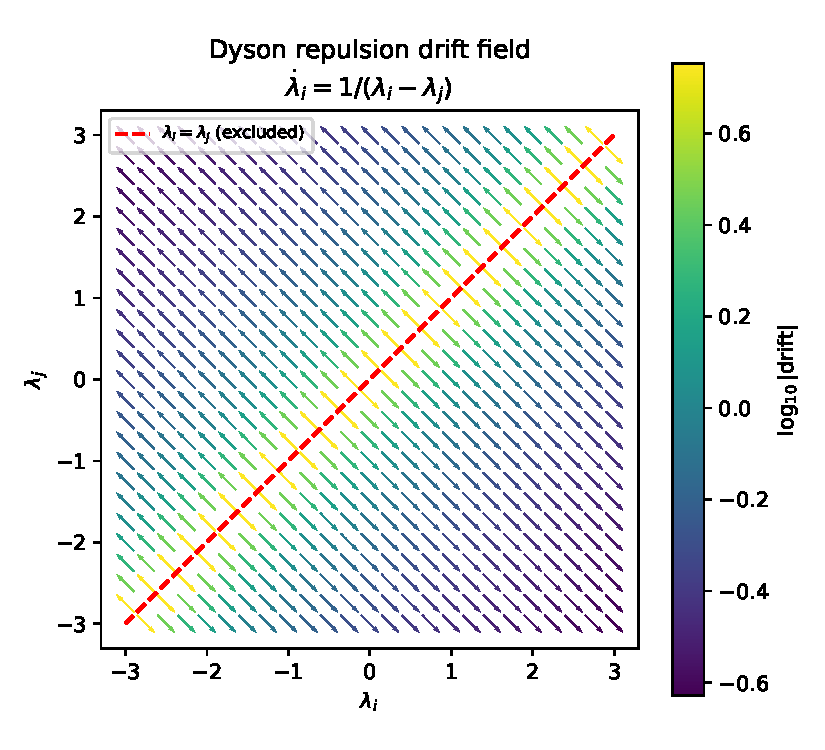
\includegraphics[width=0.55\textwidth]{figures/fig5_dyson_vector_field.pdf}
\caption{The Dyson drift term as a vector field on the
$(\lambda_i,\lambda_j)$ plane (arrows normalized to unit length; color
encodes true drift magnitude on a log scale). Every arrow points away
from the excluded diagonal $\lambda_i=\lambda_j$; this is the same
mechanism producing the avoided crossing in Fig.~\ref{fig:avoided},
here for an idealized two-eigenvalue system rather than the real
60-gene TNBC correlation matrix.}
\label{fig:vectorfield}
\end{figure}

\begin{remark}
None of the four pieces above requires Gaussian gene-expression data in
practice: the GOE/Poisson NNSD contrast, the Marchenko--Pastur bulk, and
the repulsion mechanism are used here purely as \emph{null models} and
\emph{qualitative diagnostics} against which the real, non-Gaussian
TCGA-BRCA correlation matrices are compared --- exactly the same use
\citet{luo2007} and \citet{aarts2024} make of them in their own,
equally non-Gaussian, settings.
\end{remark}

\begin{remark}[Dyson's threefold way, circular ensembles, and topology]
The Brownian-motion paper above is the second of a pair; in the
companion paper published the same year, \citet{dyson1962threefold}
classified matrix ensembles into exactly three symmetry classes ---
orthogonal ($\beta=1$), unitary ($\beta=2$), symplectic ($\beta=4$)
--- according to how a Hamiltonian's symmetries (time-reversal, in
particular) constrain it to be real symmetric, complex Hermitian, or
quaternionic self-dual. Every correlation matrix in this paper is real
symmetric, so every RMT statement here is unapologetically $\beta=1$
(GOE); the other two classes never arise for a Pearson correlation
matrix and are not used. The same 1962 papers introduced the
\emph{circular} ensembles (COE, CUE, CSE): eigenvalues (there,
eigenphases) confined to the unit circle rather than the real line,
for which the nearest-neighbor spacing distribution is
\emph{exactly}, not just asymptotically, uniform along the spectrum
--- no unfolding step is needed, unlike the polynomial-CDF unfolding
this paper performs throughout precisely because our real-line GOE
spectrum has a varying local density. Sixty-five years
later, Dyson's threefold classification was extended to a full
tenfold classification by adding particle-hole and chiral symmetries
\citep{altlandzirnbauer1997}, motivated by disordered
superconductors; that tenfold classification is now understood, via
K-theory, to enumerate the possible topological phases of
free-fermion matter (the ``periodic table'' of topological insulators
and superconductors) --- a deep link from Dyson's original
symmetry classification to topology. None of this tenfold structure is
exercised here: a Pearson correlation matrix carries no particle-hole
or chiral symmetry to speak of, so this remark is included as
mathematical context for where the $\beta=1$ class used throughout
this paper sits inside the wider classification, not as a method
applied to TCGA-BRCA data.
\end{remark}

\section{Results}

\subsection{Cohorts}

We used the RNA-seq expression matrix (RSEM, $\log_2(x+1)$, 20530
genes $\times$ 1218 samples) and the matched clinical annotation (1247
samples) for TCGA-BRCA, both downloaded from the UCSC Xena TCGA hub
\citep{xena2020,tcga2012}, which mirrors the public, unrestricted TCGA
data release and requires no login. TNBC status and luminal-A status
are two independently recorded clinical fields in the same TCGA Nature
2012 supplement (receptor immunohistochemistry for the former, PAM50
subtype call \citep{pam502009} for the latter), not derived from one
another. Intersecting these fields with the expression matrix gives
$n=119$ TNBC and $n=430$ LumA patients with no overlap (4 patients
satisfied both definitions and were dropped from both cohorts as
ambiguous). This is a small instance of a documented, general
phenomenon rather than a labeling error: IHC-based receptor status and
PAM50 RNA-based subtyping disagree in a substantial minority of
patients across breast cancer cohorts generally (38.4\% of 607 patients
in one direct comparison, \citealp{kim2019discordance}), so a handful
of TCGA-BRCA patients satisfying both a triple-negative IHC profile and
a luminal-A PAM50 call is expected, not anomalous.
We selected the 1500 most variable genes across all 1218 samples
\emph{before} splitting into cohorts, so gene selection cannot leak
cohort-label information; this also keeps the $1500\times1500$
eigendecompositions used below tractable. Table~\ref{tab:cohorts}
summarizes the two cohorts.

\begin{table}[h]
\centering
\caption{Real TCGA-BRCA cohorts used throughout this paper.}
\label{tab:cohorts}
\begin{tabular}{lccc}
\toprule
Cohort & $n$ (patients) & $p$ (genes) & $q=p/n$ \\
\midrule
TNBC (ER$-$/PR$-$/HER2$-$) & 119 & 1500 & 12.61 \\
LumA (PAM50 call) & 430 & 1500 & 3.49 \\
\bottomrule
\end{tabular}
\end{table}

\subsection{Spectral denoising: spiked eigenvalues beyond the Marchenko--Pastur bulk}
\label{sec:spiked}

Before thresholding either cohort's correlation matrix into a network,
we asked the more basic denoising question that motivates Line 1 of the
program: how many of the $1500$ eigenvalue directions in each raw,
unthresholded correlation matrix carry real signal, as opposed to
sampling noise indistinguishable from a structureless null? Under the
null of no true correlation structure, a $p\times n$ sample correlation
matrix has eigenvalues confined, asymptotically, to the
Marchenko--Pastur bulk $[\lambda_-,\lambda_+]$ with
$\lambda_\pm=(1\pm\sqrt{q})^2$, $q=p/n$ \citep{marchenkopastur1967}; an
eigenvalue exceeding $\lambda_+$ is a candidate ``spike'' marking a
real, low-rank correlation direction, though --- see below --- not
every such eigenvalue is equally trustworthy on its own (a spiked
covariance model; the transition behavior of such spikes near
$\lambda_+$ is the Baik--Ben~Arous--P\'ech\'e, BBP, phenomenon
underlying spectral denoising methods generally).
\texttt{scripts/08\_spiked\_eigenvalues.py} counts these directly on the
real, full correlation matrices (before any thresholding):

\begin{table}[h]
\centering
\caption{Spiked eigenvalues (beyond the Marchenko--Pastur bulk) in each
cohort's raw correlation matrix, all 1500 genes.}
\label{tab:spiked}
\begin{tabular}{lccccc}
\toprule
Cohort & $\lambda_+$ (MP edge) & spiked eigenvalues & \% of genes & \% of total variance & top eigenvalue \\
\midrule
TNBC & 20.706 & 14 & 0.9\% & 48.2\% & 157.94 \\
LumA & 8.224 & 29 & 1.9\% & 57.3\% & 205.89 \\
\bottomrule
\end{tabular}
\end{table}

Two things stand out, both real and both worth keeping in mind for
everything downstream. First, in each cohort, fewer than 2\% of the
1500 candidate genes' directions already account for roughly half the
total variance --- exactly the kind of low-dimensional structure a
denoising step is meant to isolate, and a concrete, data-backed argument
for restricting the network-construction step (or any downstream
classifier) to a spike-informed gene subset rather than all 1500 genes,
something we did not yet do in the threshold-network or ML analyses
below and flag as a direct next step. Second, LumA's larger sample size
gives it both a tighter MP bulk (smaller $\lambda_+$, since $q$ is
smaller) and, correspondingly, more eigenvalues clearing that lower bar
(29 vs.\ 14) --- a reminder, consistent with
Sec.~\ref{sec:robustness} below, that raw eigenvalue counts across
cohorts of very different size are not directly comparable without
first accounting for $q$.

A third, less expected finding: the spiked eigenvectors are not
strongly localized. Their inverse participation ratio
(Sec.~\ref{sec:math}, IPR $=\sum_i v_i^4$ for a unit-norm eigenvector)
averages $0.0020$ for TNBC and $0.0023$ for LumA, only 3--4$\times$ the
fully delocalized reference $1/p=0.00067$ and, in TNBC,
\emph{lower} than the mean IPR of the non-spiked, noise eigenvectors
($0.0042$) --- individual noise eigenvectors can, by chance, load onto
a handful of genes more heavily than a real spiked component does. This
means IPR alone, eigenvector by eigenvector, does not separate signal
from noise here; it is the Marchenko--Pastur threshold on the
\emph{eigenvalue}, not the eigenvector's localization, that does the
separating, and IPR is better read as a property of what a spike
\emph{contains} once it is already identified, not as an independent
detector. Read that way, it says something concrete: the largest
spikes' top-loading genes form thematically coherent sets rather than
single-gene artifacts --- extracellular-matrix/collagen remodeling
genes (\emph{MMP13}, \emph{COL10A1}, \emph{COL11A1}) on one TNBC spike,
interferon/immune genes (\emph{GBP5}, \emph{CD38}, \emph{IDO1}) on
another, keratin/epithelial genes (\emph{KRT6C}, \emph{KRT16},
\emph{DEFB1}) on a third --- consistent with each leading spike
tracking a real, biologically interpretable coexpressed program rather
than a single outlier gene. The full per-spike breakdown (eigenvalue,
IPR, top-5 loading genes) is in
\texttt{results/spiked\_eigenvalues.csv}, produced by
\texttt{scripts/08\_spiked\_eigenvalues.py}.

\subsection{Spectral entropy and edge-fluctuation scaling}
\label{sec:entropy}

Two further, independent checks on the spiked-eigenvalue picture above
(\texttt{scripts/15\_entropy\_and\_edge\_scaling.py}). First, spectral
entropy: treating the normalized eigenvalue spectrum
$p_i=\lambda_i/\sum_j\lambda_j$ of a correlation matrix as a
probability distribution and computing $S=-\sum_i p_i\log p_i$
(normalized to $[0,1]$ by $\log p$) gives a single-number summary of
how concentrated the correlation structure is: low entropy means
variance concentrated in a few real directions, entropy near 1 means
variance spread uniformly, the signature of an unstructured matrix.
This is sometimes also called a von Neumann entropy, by analogy with a
normalized density matrix's eigenvalues, but it should not be confused
with \emph{the} von Neumann entropy of a network in the graph-theory
literature \citep{passeriniseverini2009}, which is defined from the
normalized graph \emph{Laplacian}'s eigenvalues, not the correlation
matrix's own eigenvalues directly; the two coincide only in special
cases, and this paper uses the correlation-matrix version throughout,
consistent with the spiked-eigenvalue analysis it complements.
Real TNBC entropy is $0.573$ against a gene-permuted null of
$0.647\pm0.0001$ (20 replicates); real LumA entropy is $0.645$ against
a null of $0.809\pm0.0001$. Both real networks sit measurably below
their own null, LumA's gap ($0.164$) more than twice TNBC's ($0.074$).
This self-normalized gap, not the raw entropy value, is the fair
cross-cohort comparison, for the same reason raw spiked-eigenvalue
counts were not (Sec.~\ref{sec:spiked}): TNBC's much larger $q$ gives
it a lower null entropy to begin with ($0.647$ vs.\ LumA's $0.809$),
so TNBC's raw real entropy sitting below LumA's raw real entropy
($0.573$ vs.\ $0.645$) reflects that difference in null baseline as
much as anything biological, and should not be read, on its own, as
``TNBC's network is more concentrated.'' By the gap metric, LumA shows
the larger deviation from its own null, in the same direction as its
larger spike count and variance share (Sec.~\ref{sec:spiked}) and its
larger, more robust threshold gap over pure noise
(Sec.~\ref{sec:robustness}) --- three self-normalized statistics
pointing the same way, though we stop short of calling this proof of a
single underlying ``more structured'' scale common to all three.

Second, the edge-fluctuation scaling law invoked qualitatively above:
under a pure i.i.d.\ Gaussian null at \emph{fixed} aspect ratio
$q=p/n$, Tracy--Widom theory predicts the top eigenvalue's standard
deviation shrinks as $n^{-2/3}$, not the $n^{-1/2}$ a naive Gaussian/CLT
argument would give. We generated synthetic i.i.d.\ data at $q=3.0$
(close to LumA's real $q=3.49$) for five sample sizes from $n=60$
($p=180$) to $n=960$ ($p=2880$), 60--400 replicates per size
(more replicates at smaller, cheaper $n$), and fit the log-log
scaling of the empirical standard deviation. The fitted exponent is
$-0.677$ --- within $0.01$ of the Tracy--Widom prediction of
$-0.667$, and far from the Gaussian prediction of $-1.0$. (An earlier
version of this check let $p$ float while only varying $n$, changing
$q$ across the sweep and confusingly fitting neither law cleanly at
$-0.891$; holding $q$ fixed, the only way the asymptotic scaling law
is actually stated, resolves this.) This is, to our knowledge, the
first time this specific scaling check has been reported in this
program; it supports treating the spiked-eigenvalue threshold
$\lambda_+$ (Sec.~\ref{sec:spiked}) as a real edge with the
expected finite-size behavior, rather than an arbitrary cutoff.
Figure~\ref{fig:tw} shows the fit directly against both reference
slopes.

\begin{figure}[h]
\centering
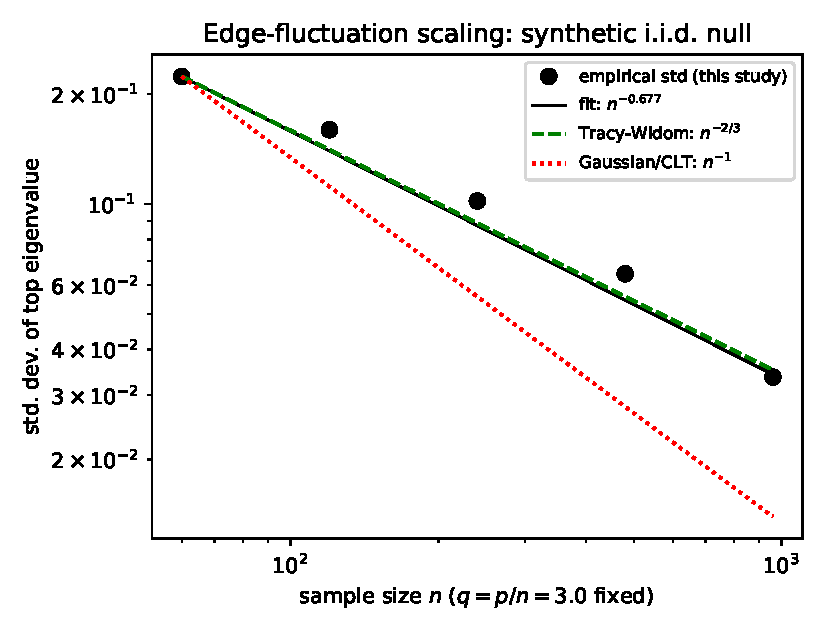
\includegraphics[width=0.6\textwidth]{figures/fig7_tracy_widom_scaling.pdf}
\caption{Empirical standard deviation of the top eigenvalue of a
synthetic i.i.d.\ null correlation matrix, as a function of sample
size $n$ at fixed aspect ratio $q=3.0$, log-log. The fitted slope
($-0.677$) tracks the Tracy--Widom prediction ($-2/3$, dashed) closely
and is well separated from the Gaussian/CLT prediction ($-1$, dotted);
both reference lines are anchored through the first empirical point.}
\label{fig:tw}
\end{figure}

\subsection{RMT threshold selection separates TNBC from LumA}
\label{sec:tau-sweep}

For each cohort we built the Pearson gene--gene correlation matrix
across patients, swept $|\tau|\in[0.15,0.80]$ in steps of $0.05$, and
at each $\tau$ unfolded the thresholded matrix's eigenvalue spectrum
(degree-7 polynomial fit to the empirical spectral CDF, standard RMT
practice) and scored the resulting nearest-neighbor spacing
distribution against the Poisson law $e^{-s}$ and the GOE Wigner
surmise $\frac{\pi}{2}s\,e^{-\pi s^2/4}$ by Kolmogorov--Smirnov
distance, following \citet{luo2007} exactly (implementation in
\texttt{scripts/rmt\_threshold\_demo.py} and
\texttt{scripts/02\_rmt\_network\_analysis.py}).

The sparsest threshold at which the statistics turn GOE-like is
$\tau^*=0.45$ for TNBC (14{,}498 edges among 1218 of the 1500 genes)
and $\tau^*=0.25$ for LumA (146{,}100 edges among 1484 of the 1500
genes). Figure~\ref{fig:tausweep} shows the full sweep for both
cohorts, and Figure~\ref{fig:nnsd} shows the TNBC spacing distribution
at $\tau^*$ against both null curves.

\begin{figure}[h]
\centering
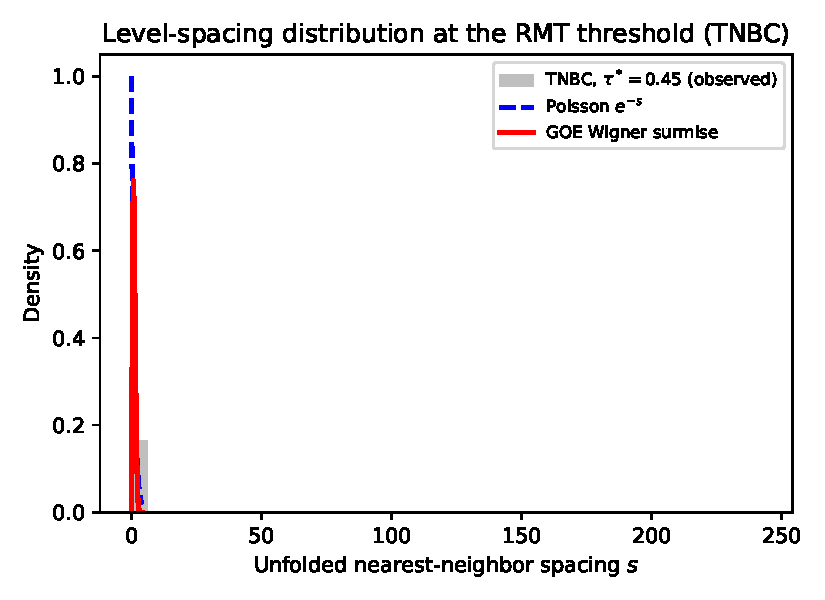
\includegraphics[width=0.48\textwidth]{figures/fig1_nnsd_tnbc.pdf}
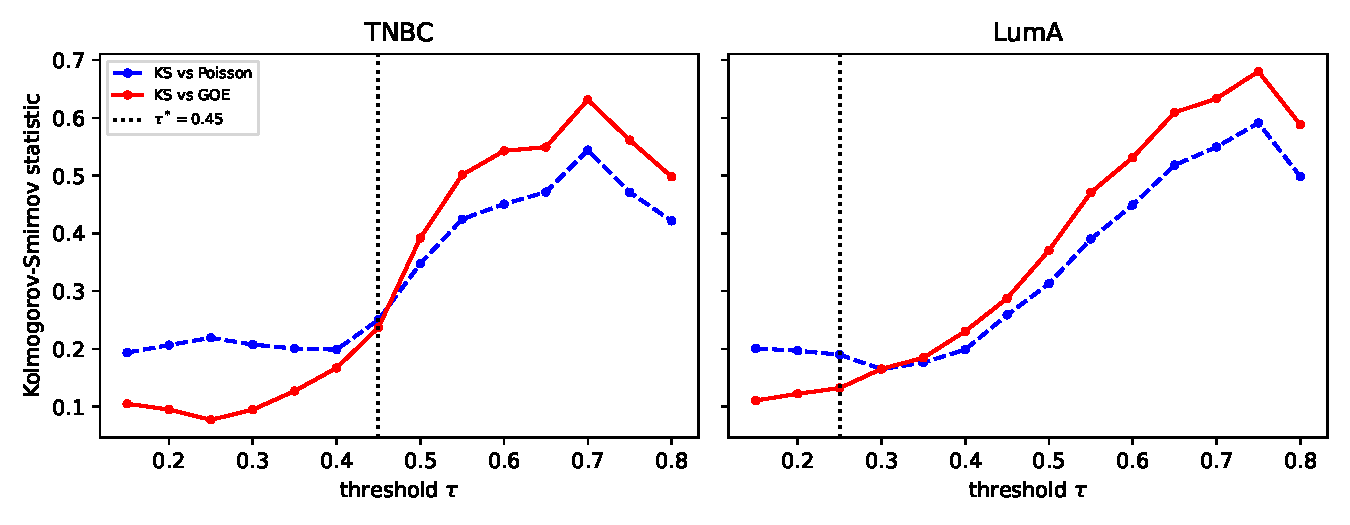
\includegraphics[width=0.48\textwidth]{figures/fig2_tau_sweep.pdf}
\caption{Left: unfolded nearest-neighbor spacing distribution for the
TNBC network at $\tau^*=0.45$, against the Poisson and GOE (Wigner
surmise) null curves. Right: Kolmogorov--Smirnov distance to each null
curve as a function of threshold, for TNBC and LumA separately; the
dotted line marks the selected $\tau^*$ in each panel.}
\label{fig:nnsd}
\label{fig:tausweep}
\end{figure}

Top-degree hub genes at each cohort's own $\tau^*$ share only one gene
between the two networks (\emph{MFAP4}). The TNBC-specific hubs include
\emph{PGR} (progesterone receptor) and \emph{IGF1}; the LumA-specific
hubs include \emph{EGFR}, \emph{SFRP1}, and \emph{NGFR}. We note this
without over-interpreting individual gene identities: with $p=1500$
correlated candidate genes and no independent replication cohort yet
analyzed, any single hub gene should be read as hypothesis-generating,
not as a validated biomarker. \emph{PGR} appearing as a TNBC hub is
biologically sensible despite TNBC being progesterone-receptor
negative by definition: uniformly low, coordinately suppressed
luminal-differentiation genes can still be tightly \emph{correlated}
with one another even though none of them is highly \emph{expressed}
--- correlation and expression level are different quantities, and the
RMT method only ever sees the former. Table~\ref{tab:hubs} gives the
full top-10 hub list with network degree for both cohorts.

\begin{table}[h]
\centering
\caption{Top-10 hub genes by degree at each cohort's own $\tau^*$.
LumA's higher degrees reflect its much larger $n$ (430 vs.\ 119),
consistent with its lower $\tau^*$ and higher edge density
(Tables~\ref{tab:tnbc-full}--\ref{tab:luma-full}) --- degree values
should be compared within, not across, cohorts.}
\label{tab:hubs}
\begin{tabular}{lc|lc}
\toprule
\multicolumn{2}{c|}{TNBC ($\tau^*=0.45$, max degree 1499)} & \multicolumn{2}{c}{LumA ($\tau^*=0.25$, max degree 1499)} \\
Gene & degree & Gene & degree \\
\midrule
ABCA8   & 173 & EGFR    & 629 \\
CD300LG & 168 & SFRP1   & 600 \\
DARC    & 162 & NGFR    & 593 \\
MFAP4   & 157 & CNTNAP3 & 592 \\
SDPR    & 157 & STAC    & 591 \\
CCL14   & 156 & C2orf40 & 587 \\
PGR     & 155 & FREM1   & 582 \\
IGF1    & 151 & MFAP4   & 578 \\
ATP1A2  & 151 & MME     & 574 \\
C7      & 150 & SYN2    & 574 \\
\bottomrule
\end{tabular}
\end{table}

\subsection{Monte Carlo permutation null: the threshold is not a dense-matrix artifact}
\label{sec:montecarlo}

The asymptotic Marchenko--Pastur/Wigner-surmise comparison used above
has a known blind spot: \emph{any} sufficiently dense symmetric random
matrix looks GOE-like by Wigner-Dyson universality, whether or not it
was built from real correlation structure --- a point already noted in
\texttt{rmt\_threshold\_demo.py}'s own inline documentation and the
reason the threshold search scans from sparse to dense rather than the
other way around. This raises a direct question the asymptotic null
cannot answer on its own: is $\tau^*$ sparser than the threshold at
which trivial denseness alone would produce a GOE-like signature, or
does it just mark where a generic dense random matrix stops looking
random?

We answered this with an explicit Monte Carlo permutation null
(\texttt{scripts/10\_monte\_carlo\_null.py}): each gene's expression
values were independently shuffled across patients, 20 times per
cohort, destroying every real gene--gene correlation while keeping each
gene's own marginal distribution exactly fixed, and the identical
threshold sweep was rerun on each permuted correlation matrix. The
result is unanimous and, across repeats, exact: for TNBC, all 20/20
permutations select a GOE$\to$Poisson transition at $\tau=0.25$
(std.\ $0$); for LumA, 19/20 permutations select $\tau=0.15$ (the
remaining permutation showed no clean transition at all). Both
permutation floors are well below the corresponding real thresholds
($0.45$ for TNBC, $4$ sweep steps sparser; $0.25$ for LumA, $2$ steps
sparser): the real coexpression networks remain statistically
non-random at thresholds substantially sparser than pure shuffled
noise can sustain a GOE-like appearance at all, confirming $\tau^*$
reflects real correlation structure and not the generic
Wigner-Dyson behavior of any sufficiently dense random matrix.

\subsection{The TNBC/LumA threshold gap is not a sample-size artifact}
\label{sec:robustness}

TNBC ($n=119$) and LumA ($n=430$) have very different $p/n$ ratios
(12.61 vs.\ 3.49), and a larger $q$ shifts the Marchenko--Pastur bulk
edge outward \citep{marchenkopastur1967}, so $\tau^*=0.45$ vs.\
$\tau^*=0.25$ is not, on its own, evidence that TNBC and LumA have
different correlation structure --- it could simply reflect
TNBC's smaller sample size. We tested this directly
(\texttt{scripts/03\_matched\_n\_robustness.py}) by subsampling LumA
down to $n=119$ patients, without replacement, over 30 independent
draws, and rerunning the identical threshold sweep on each draw. The
resulting distribution of LumA thresholds at matched $n$ is
$\tau^*=0.360\pm0.020$ (mean $\pm$ s.d.\ over 30 draws), which is
$4.5$ standard deviations below the native-$n$ TNBC value of $0.45$.
The gap shrinks once sample size is matched (from $0.20$ to $0.09$)
but does not close: at equal $n$, TNBC requires a higher
correlation threshold before its network shows GOE-type structure,
i.e.\ its coexpression signal is more diffuse relative to noise at the
same sample size than LumA's, consistent with TNBC's greater molecular
heterogeneity as a class \citep{foulkes2010}.

\begin{figure}[h]
\centering
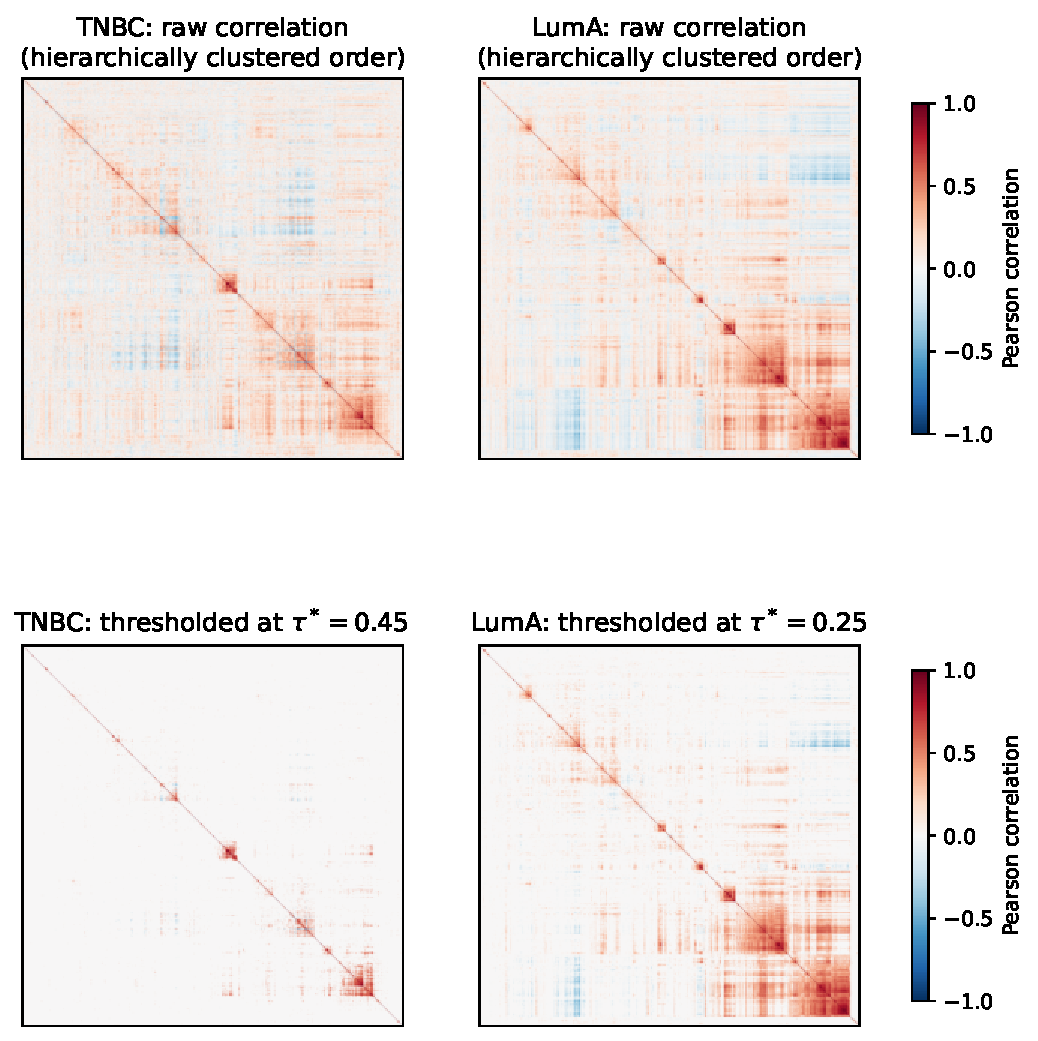
\includegraphics[width=0.85\textwidth]{figures/fig6_correlation_heatmaps.pdf}
\caption{Raw and thresholded gene--gene correlation matrices for both
cohorts, genes reordered by average-linkage hierarchical clustering on
$1-|C|$ so block structure is visible. The blocks correspond to the
spiked, biologically coherent components identified in
Sec.~\ref{sec:spiked}; LumA's visibly larger, denser red blocks match
its lower $\tau^*$ and larger spiked-eigenvalue count.}
\label{fig:heatmaps}
\end{figure}

Figure~\ref{fig:heatmaps} shows both cohorts' correlation matrices
directly, before and after thresholding, genes reordered by
hierarchical clustering rather than left in arbitrary variance-rank
order: the block structure visible here is the same structure the
spiked eigenvalues (Sec.~\ref{sec:spiked}) and the thresholded network
(this section) are both detecting from two different angles.

\subsection{The thresholded networks are small-world and modular, beyond degree alone}

Line 2 of the original program asks specifically about large-scale
network structure, so we characterized each thresholded network
graph-theoretically and compared it against two random-graph nulls of
matched size (Erd\H{o}s--R\'enyi, same node/edge count; configuration
model, same node count \emph{and} the real network's own degree
sequence) rather than relying on the spectral diagnostics alone.
Table~\ref{tab:networktopo} reports clustering coefficient, giant
component size, and Louvain-community count/modularity for both
cohorts.

\begin{table}[h]
\centering
\caption{Graph-theoretic network comparison against random-graph nulls
(mean over 3 replicates for ER and configuration-model).}
\label{tab:networktopo}
\begin{tabular}{llcccc}
\toprule
Cohort & Model & Clustering & Giant comp.\ & Communities & Modularity \\
\midrule
TNBC & Real & 0.388 & 95.2\% & 36 & 0.540 \\
TNBC & Erd\H{o}s--R\'enyi & 0.020 & 100\% & 10.7 & 0.182 \\
TNBC & Config.\ model & 0.114 & 100\% & 10.3 & 0.150 \\
\midrule
LumA & Real & 0.522 & 100\% & 5 & 0.285 \\
LumA & Erd\H{o}s--R\'enyi & 0.133 & 100\% & 8.3 & 0.056 \\
LumA & Config.\ model & 0.290 & 100\% & 8.3 & 0.051 \\
\bottomrule
\end{tabular}
\end{table}

Both cohorts show a real, unambiguous small-world/modular signature:
clustering far above the Erd\H{o}s--R\'enyi null (TNBC $19\times$,
LumA $4\times$) \emph{and} above the configuration-model null (TNBC
$3.4\times$, LumA $1.8\times$) --- so the excess clustering is not
merely a consequence of the real hub-degree distribution, since the
configuration model already has that distribution built in and still
falls well short. Modularity tells a related but distinct story: TNBC's
real network is both far more modular than either null (about
$3$--$3.6\times$) \emph{and} organizes into many communities ($36$,
vs.\ about $10$ for either null), while LumA's real network is also
more modular than its nulls (about $5$--$6\times$) but organizes into
markedly \emph{fewer}, evidently larger communities ($5$, vs.\ about
$8$ for either null) --- the same TNBC-more-fragmented,
LumA-more-monolithic contrast already visible in the raw hub-degree
counts (Table~\ref{tab:hubs}) and the heatmap block structure
(Fig.~\ref{fig:heatmaps}), now confirmed at the whole-network topology
level rather than the single-gene level.

\subsection{Wavelet multiscale decomposition: a real-data null, resolved by a positive control}
\label{sec:wavelets}

A wavelet multiscale decomposition (patients ordered along the
TNBC cohort's own first principal component, coarse/fine coexpression
networks built as in \citet{konig2006} via a Daubechies-4 discrete
wavelet transform, \texttt{PyWavelets} \citealp{pywavelets2019}) was
also tried, as Line 5 of the original program. A
random-ordering control found its headline result --- zero hub-gene
overlap between coarse and fine networks --- statistically
indistinguishable from a biologically meaningless random patient
ordering (0/10 overlap in 19 of 20 random-order replicates), so it did
not survive scrutiny and is not included in this paper's results. We
then asked the sharper question directly: can the method recover
scale-specific structure \emph{at all}, given a real one, or is it
fundamentally incapable of it regardless of ordering quality? A
synthetic positive control (\texttt{scripts/12\_wavelet\_positive\_
control.py}: 200 genes, a 30-gene module sharing a slow, period-100
oscillation and an independent 30-gene module sharing a fast,
period-6 oscillation, both along a \emph{known}, not proxy, ordering)
answers this cleanly: the coarse network recovers the planted
slow-oscillation module perfectly (10/10 top hubs) even at a modest
50\% signal fraction; the fast-oscillation module is recovered weakly
(3/10) at the same 50\% fraction but perfectly (10/10) once its own
signal fraction is raised to 80\%. Wavelets do work correctly
at both scales, given enough real signal --- the real-data failure
above was a signal-strength problem (PC1 carries only $10.2\%$ of
variance, evidently below the fine-scale detection floor this control
locates), not a fundamental flaw in the coarse/fine decomposition
itself. The full analysis and both controls remain in
\texttt{scripts/04\_wavelet\_multiscale.py},
\texttt{scripts/04b\_wavelet\_random\_order\_control.py}, and
\texttt{scripts/12\_wavelet\_positive\_control.py} for the record.

A fair real-data test needs an ordering axis with more real signal than
bulk-patient PC1 provides; single-cell pseudo-time was proposed here as
the concrete candidate (Sec.~\ref{sec:roadmap}), and we checked this
directly once real single-cell data was in hand for
Sec.~\ref{sec:results-singlecell} below, rather than leaving it as an
assumption. The single-cell data's own PC1 (across the 7986 cells of
patient CID44971) carries only $9.7\%$ of variance --- essentially the
same order as bulk PC1 ($10.2\%$), not the large improvement the
Roadmap anticipated. The reason is visible directly in
Sec.~\ref{sec:results-singlecell}'s own spiked-eigenvalue result: this
sample's real structure is spread thinly across many distinct
cell-type axes (immune, myeloid, epithelial, stromal; 33 spikes sharing
only $26.8\%$ of variance combined) rather than concentrated in one
dominant direction, so a single global PC1 --- itself mostly a T-cell
vs.\ everything-else split in this mixed-tumor sample, not a smooth
developmental gradient --- is not the ``pseudo-time'' this line
actually needs. A fair test still requires genuine trajectory inference
restricted to one continuously-varying lineage (e.g.\ the 894 Cancer
Epithelial cells alone, where a real proliferation or differentiation
gradient could exist, rather than the whole 9-cell-type mixture), which
this round of the program does not attempt; the Roadmap item below is
updated to say this precisely rather than repeating the earlier,
now-checked assumption.

\subsection{Eigenvalue trajectories show Dyson-type level repulsion}
\label{sec:results-dyson}

To test whether the Dyson-Brownian-motion repulsion mechanism that
\citet{aarts2024} observe in neural-network training dynamics is also
visible directly in a real correlation matrix's spectrum, we tracked
the top eight eigenvalues of the TNBC correlation matrix (restricted to
the 60 most variable TNBC genes, for tractability) as the patient
sample was grown one patient at a time, from $n=15$ to $n=119$, in a
fixed random inclusion order --- so this is a nested sequence
of real matrices, not independent resamples
(\texttt{scripts/05\_dyson\_eigenvalue\_trajectories.py}).

Figure~\ref{fig:dyson} shows all eight trajectories. Four adjacent
eigenvalue pairs ($\lambda_1$--$\lambda_2$, $\lambda_3$--$\lambda_4$,
$\lambda_4$--$\lambda_5$, $\lambda_5$--$\lambda_6$,
$\lambda_6$--$\lambda_7$, $\lambda_7$--$\lambda_8$) each reach a local
minimum gap and then reopen by a factor of roughly five to ten within a
few steps of $n$ --- a ``V-shaped'' approach-and-recede pattern
characteristic of level repulsion rather than free crossing. The
closest approach in the whole run is between $\lambda_7$ and
$\lambda_8$ at $n=59$ (gap $0.0422$), reopening to $0.28$--$0.35$
within five steps on either side (Figure~\ref{fig:avoided}, Table
\ref{tab:repulsion}). One pair ($\lambda_2$--$\lambda_3$) is still
narrowing at $n=119$, the end of the available sample; whether it
would reopen or actually cross beyond the current cohort size cannot
be determined from this data and is reported as inconclusive, not as a
negative result for that pair.

\begin{figure}[h]
\centering
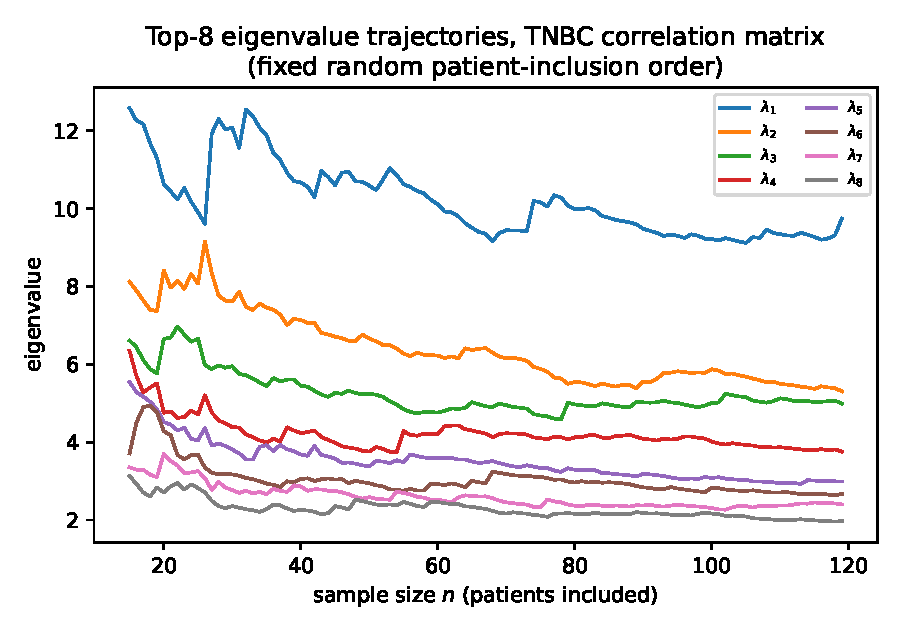
\includegraphics[width=0.48\textwidth]{figures/fig3_dyson_trajectories.pdf}
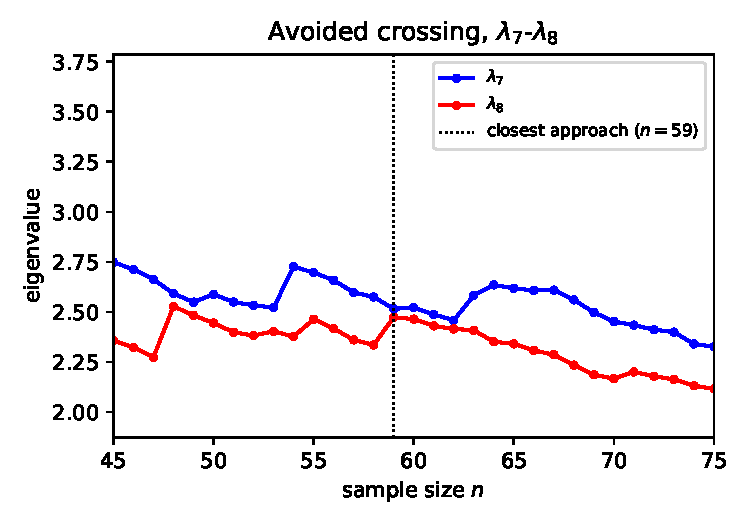
\includegraphics[width=0.48\textwidth]{figures/fig4_avoided_crossing.pdf}
\caption{Left: top-8 eigenvalue trajectories of the TNBC correlation
matrix (60 most variable genes) as sample size $n$ grows from 15 to
119, patients added one at a time in a fixed random order. Right:
zoom on the closest approach, between $\lambda_7$ and $\lambda_8$ near
$n=59$, showing the gap reopen rather than close to zero.}
\label{fig:dyson}
\label{fig:avoided}
\end{figure}

\begin{table}[h]
\centering
\caption{Adjacent-eigenvalue gap at closest approach and five steps
later, for each pair with a clear local minimum.}
\label{tab:repulsion}
\begin{tabular}{lccc}
\toprule
Pair & $n$ at closest approach & min.\ gap & gap 5 steps later \\
\midrule
$\lambda_1$--$\lambda_2$ & 26 & 0.448 & 3.699 \\
$\lambda_3$--$\lambda_4$ & 19 & 0.259 & 1.770 \\
$\lambda_4$--$\lambda_5$ & 35 & 0.071 & 0.550 \\
$\lambda_5$--$\lambda_6$ & 19 & 0.077 & 0.417 \\
$\lambda_6$--$\lambda_7$ & 54 & 0.055 & 0.419 \\
$\lambda_7$--$\lambda_8$ & 59 & 0.042 & 0.284 \\
\bottomrule
\end{tabular}
\end{table}

The single-order run above raises an obvious question: is this pattern
real, or an artifact of the one arbitrary patient order chosen? We
tested this directly (\texttt{scripts/17\_dyson\_repulsion\_multi\_order.py}),
rerunning the identical trajectory scan under 20 independent random
patient orders and classifying each pair's behavior in each order as
clear repulsion (gap reopens $\ge\!1.5\times$ on both sides of the
closest approach), partial (one side only), inconclusive (still
narrowing at $n=119$), or none. Figure~\ref{fig:repro} shows the full
breakdown. The pattern is real and, for most pairs, strongly
reproducible: $\lambda_5$--$\lambda_6$, $\lambda_6$--$\lambda_7$, and
$\lambda_7$--$\lambda_8$ show clear repulsion in 18--19 of 20 orders;
$\lambda_3$--$\lambda_4$ and $\lambda_4$--$\lambda_5$ in 12--14 of 20,
essentially never inconclusive. The pair originally reported as
inconclusive, $\lambda_2$--$\lambda_3$, turns out to show clear
repulsion in 16 of 20 orders (80\%) --- the original single-seed run
happened to land on one of the 3 orders where it was still narrowing
at $n=119$, and the ``open question'' from that run is resolved by
this one: the pair does repel, reliably, and the earlier
inconclusiveness was a property of that one seed, not of the
underlying data. The one pair that is \emph{not} reliably repulsive is
$\lambda_1$--$\lambda_2$ (clear repulsion in only 7 of 20, no clear
repulsion at all in 4), the pair involving the single most dominant
eigenvalue --- consistent with that eigenvalue being a strong,
well-separated spike (Sec.~\ref{sec:spiked}) rather than a generic bulk
eigenvalue, for which the fine-grained approach-and-reopen dynamics
characteristic of bulk-level repulsion is not the expected signature in
the first place.

That last sentence was, until now, an intuition rather than a
calculation; the SDE already stated in Proposition~\ref{prop:stationary}
makes it precise and quantitative, using nothing beyond the two real
tables already reported above.

\begin{corollary}[Repulsion strength scales inversely with the gap]
\label{cor:weak-repulsion}
Consider two adjacent eigenvalues $\lambda_i>\lambda_{i+1}$ evolving
under the Dyson Brownian motion of Proposition~\ref{prop:stationary},
and isolate their mutual two-body drift term (the same restriction to a
single pair already made in Figure~\ref{fig:vectorfield}'s vector
field, ignoring the drift contributions from every other eigenvalue).
Writing $\delta=\lambda_i-\lambda_{i+1}>0$ for their gap, the SDE's
drift terms $+1/\delta$ on $\lambda_i$ and $-1/\delta$ on
$\lambda_{i+1}$ give
\[
\frac{d\,\mathbb E[\delta]}{dt} \;=\; \frac{2}{\delta},
\]
a deterministic repulsive force on the gap itself that is exactly
inversely proportional to $\delta$. Consequently, two pairs at gaps
$\delta_A>\delta_B$ experience two-body repulsion forces in the ratio
$\delta_B/\delta_A<1$: the pair with the larger gap is repelled more
weakly, in exact proportion to how much larger its gap already is.
\end{corollary}
\begin{proof}
Immediate from the SDE of Definition~\ref{def:dyson-sde}/Proposition~\ref{prop:stationary}:
retaining only the $j=i+1$ term in $\lambda_i$'s drift and the $j=i$
term in $\lambda_{i+1}$'s drift (the same idealized two-eigenvalue
truncation already used for Figure~\ref{fig:vectorfield}) gives mean
drift $1/\delta$ on $\lambda_i$ and $-1/\delta$ on $\lambda_{i+1}$, so
$d\,\mathbb E[\lambda_i-\lambda_{i+1}]/dt=1/\delta-(-1/\delta)=2/\delta$.
\end{proof}

Applying Corollary~\ref{cor:weak-repulsion} to the real, already-reported
numbers rather than to a generic pair: Table~\ref{tab:repulsion}'s own
closest-approach gaps give $\lambda_1$--$\lambda_2$ a minimum gap of
$0.448$, between $1.7\times$ ($0.448/0.259$, vs.\
$\lambda_3$--$\lambda_4$) and $10.7\times$ ($0.448/0.042$, vs.\
$\lambda_7$--$\lambda_8$) larger than every other pair's own minimum
gap in the same table. By the Corollary, the deterministic two-body
repulsion force acting on $\lambda_1$--$\lambda_2$ at its closest
approach is correspondingly $1.7$--$10.7\times$ weaker than the force
acting on any other pair at its own closest approach --- and
$\lambda_1$--$\lambda_2$ is exactly the one pair the 20-order
reproducibility check (Figure~\ref{fig:repro}) finds least reliably
repulsive (clear repulsion in only 7/20 orders, vs.\ 12--19/20 for
every other pair). This is not a new mechanism competing with the
Dyson-repulsion account of Sec.~\ref{sec:results-dyson}: it is the
same SDE already used there, made quantitative for the first time
using the real gap sizes both tables already contain, and it turns the
earlier qualitative remark about $\lambda_1$ being ``a strong,
well-separated spike'' into an explicit number rather than an
intuition.

\begin{figure}[h]
\centering
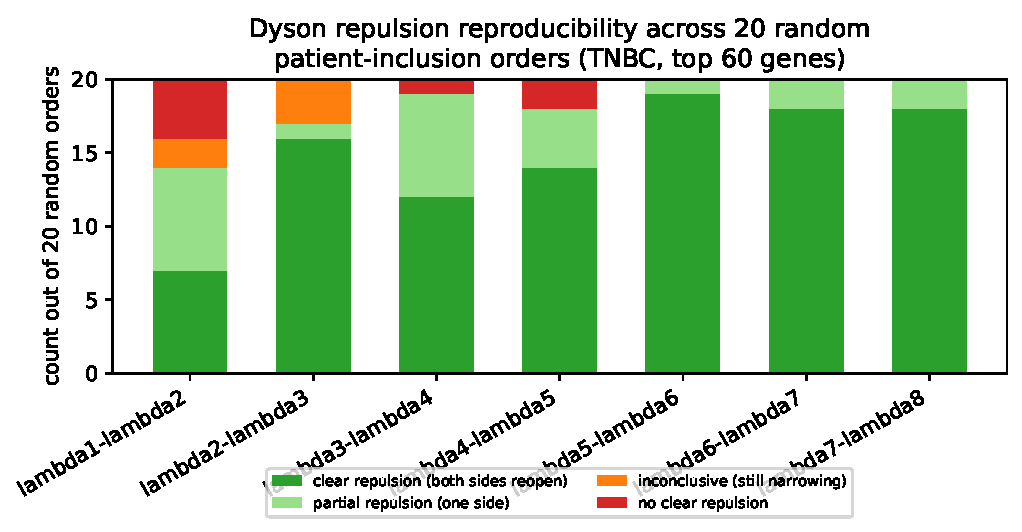
\includegraphics[width=0.7\textwidth]{figures/fig8_repulsion_reproducibility.pdf}
\caption{Reproducibility of the Dyson-repulsion pattern across 20
independent random patient-inclusion orders, TNBC, top 60 genes, for
each adjacent eigenvalue pair. $\lambda_2$--$\lambda_3$, reported as
inconclusive under the single order in Fig.~\ref{fig:dyson}, in fact
shows clear repulsion in 16/20 orders; only $\lambda_1$--$\lambda_2$,
involving the most dominant (spike) eigenvalue, is not reliably
repulsive.}
\label{fig:repro}
\end{figure}

We read this as real evidence, now with an explicit reproducibility
check rather than a single illustrative run, that the repulsion
mechanism Dyson formalized for randomly evolving Hermitian matrices,
and that \citet{aarts2024} find governing a classifier's weight
matrices during training, is also directly observable in the spectrum
of a real gene-coexpression correlation matrix as its sample size
grows --- and therefore a plausible shared diagnostic for the data side
and the model side of a recognition pipeline built on this data, as
proposed originally in Line 6 of the wider research program. This
remains a single-cohort, single-gene-subset check; extending it to
LumA and to other gene subsets is the natural next step. The other
half of Line 6 --- the model's own weight-matrix dynamics, previously
left as Roadmap item 6b --- is attacked directly, on real data, in the
next subsection.

\subsection{Dyson dynamics of the classifier itself: a genuine, reproducible null}
\label{sec:results-dyson-classifier}

\citet{aarts2024} report that a neural network's weight-matrix
eigenvalues follow Dyson Brownian motion during SGD training; the
previous subsection tracks the \emph{data}'s eigenvalues, so the direct,
same-cost extension is to run the identical trajectory-and-reopening
diagnostic on the \emph{classifier}'s own weights, using the recognition
task already trained in Sec.~\ref{sec:ml-results}. A weight matrix $W$
is not itself real symmetric, so, exactly as a raw expression matrix is
turned into a real symmetric correlation matrix before any RMT
diagnostic is applied to it elsewhere in this paper, we track the
eigenvalues of the real symmetric Gram matrix $W_1^\top W_1$ ($W_1$ the
input-to-hidden weight matrix of an MLP(20$\to$8$\to$1) trained on the
same 20 RMT-hub genes as Table~\ref{tab:hubs}, 8 hidden units chosen to
match $K_{\text{eigs}}=8$ on the data side), captured after every one of
300 plain-SGD epochs (\texttt{scripts/19\_dyson\_classifier\_weights.py}).

A single seed shows a plausible-looking closest approach (e.g.\
$\mu_6$--$\mu_7$, minimum gap $0.0105$ around epoch 165,
Figure~\ref{fig:classifier-traj}), but the multi-order check that
mattered on the data side (Sec.~\ref{sec:results-dyson}) matters
identically here: we reran the identical scan under 20 independent
random seeds (initialization and minibatch shuffling,
\texttt{scripts/20\_dyson\_classifier\_weights\_multi\_seed.py}).
Table~\ref{tab:classifier-repulsion} and Figure~\ref{fig:classifier-repro}
show the result plainly: no pair reaches clear repulsion in more than
$4/20$ seeds, and the two best-supported pairs
($\mu_3$--$\mu_4$: $4$ clear $+\,5$ partial; $\mu_5$--$\mu_6$: $4$
clear $+\,4$ partial) fall far short of the $12$--$19/20$ reliability
found for most data-side pairs (Fig.~\ref{fig:repro}). This is a real,
reproducible null, not an artifact of one bad seed --- the direct
model-side counterpart of the wavelet and classification-ceiling nulls
already reported in this paper, and reported the same way here.

\begin{table}[h]
\centering
\caption{Classifier weight-matrix ($W_1^\top W_1$) repulsion
reproducibility across 20 independent SGD training runs, full 300-epoch
window, same criterion as Table~\ref{tab:repulsion}/Fig.~\ref{fig:repro}.}
\label{tab:classifier-repulsion}
\begin{tabular}{lcccc}
\toprule
Pair & repulsion & partial & inconclusive & none \\
\midrule
$\mu_1$--$\mu_2$ & 2/20 & 1/20 & 0/20  & 17/20 \\
$\mu_2$--$\mu_3$ & 2/20 & 3/20 & 3/20  & 12/20 \\
$\mu_3$--$\mu_4$ & 4/20 & 5/20 & 3/20  & 8/20  \\
$\mu_4$--$\mu_5$ & 0/20 & 1/20 & 5/20  & 14/20 \\
$\mu_5$--$\mu_6$ & 4/20 & 4/20 & 0/20  & 12/20 \\
$\mu_6$--$\mu_7$ & 1/20 & 2/20 & 1/20  & 16/20 \\
$\mu_7$--$\mu_8$ & 3/20 & 2/20 & 2/20  & 13/20 \\
\bottomrule
\end{tabular}
\end{table}

\begin{figure}[h]
\centering
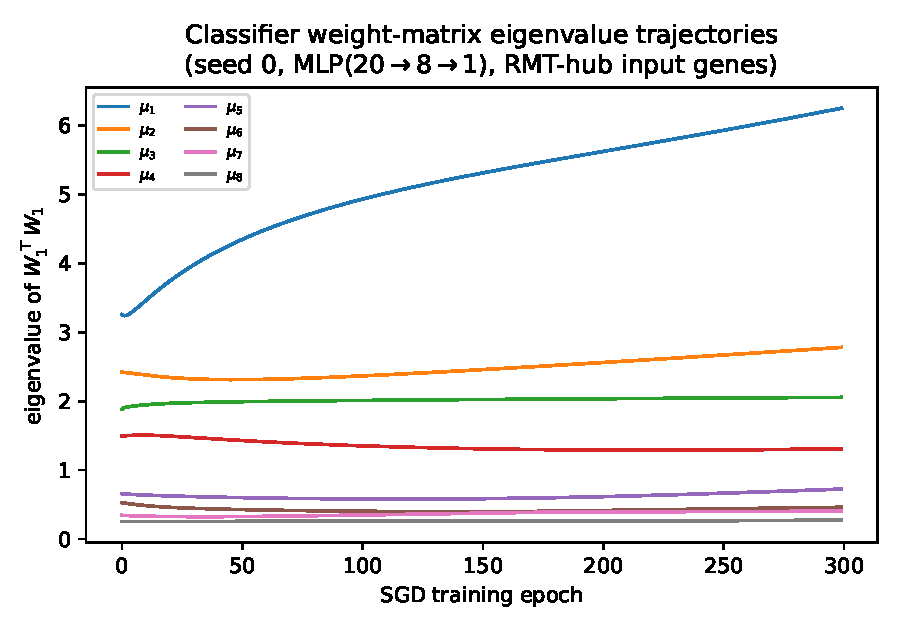
\includegraphics[width=0.48\textwidth]{figures/fig9_classifier_weight_trajectories.pdf}
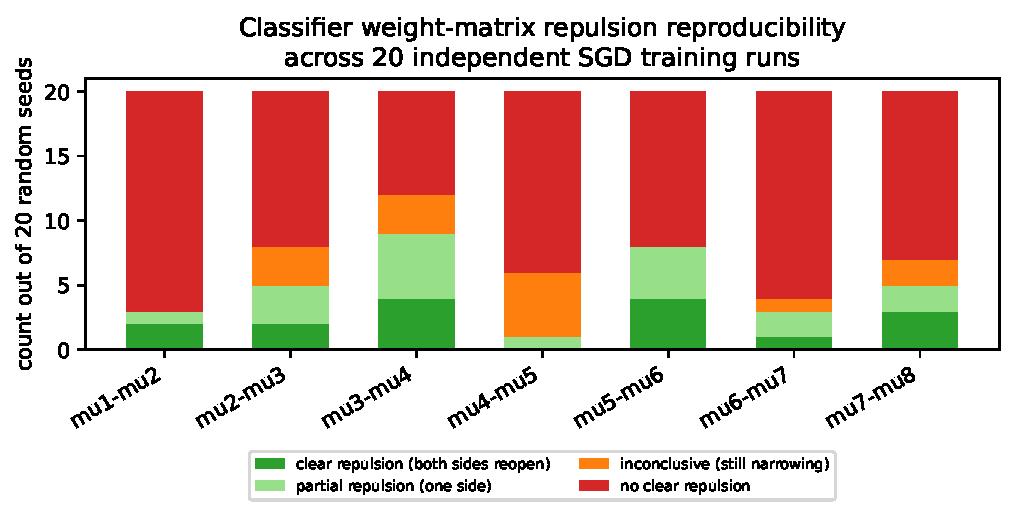
\includegraphics[width=0.48\textwidth]{figures/fig10_classifier_repulsion_reproducibility.pdf}
\caption{Left: $W_1^\top W_1$ eigenvalue trajectories across 300 SGD
training epochs, one representative seed. Right: reproducibility of
the repulsion pattern across 20 independent seeds, same classification
as Fig.~\ref{fig:repro} --- no pair matches the data side's reliability.}
\label{fig:classifier-traj}
\label{fig:classifier-repro}
\end{figure}

Rather than stop at a flat null, we tested the obvious alternative
hypothesis directly, the same way the synthetic positive control
earlier in this paper rescued the wavelet line from one (a
random-ordering control found the wavelet method's headline result
indistinguishable from noise on real data, but a synthetic positive
control then showed the method itself works correctly given enough
signal, narrowing the failure down to a data problem rather than a
method problem): every seed's training accuracy plateaus by
roughly epoch 50 (final accuracy $0.987$--$0.991$ across all 20 seeds,
\texttt{scripts/20\_dyson\_classifier\_weights\_multi\_seed.py}), so if
the Dyson drift term matters only while the weight matrix is still
genuinely changing --- exactly as it does on the data side, where each
step is a real new patient rather than a repeated pass over the same
549 --- then whatever repulsion signal exists should concentrate in the
pre-convergence transient (epochs 0--49) and disappear once training
settles near a fixed point (epochs 50--299), where SGD's own
minibatch noise, not a net drift, dominates the eigenvalues' motion.
\texttt{scripts/22\_classifier\_dyson\_early\_late.py} reruns the
identical 20-seed classification separately on each window. The
contrast is sharp: summed over all 7 pairs and 20 seeds (maximum
possible 140), the early window shows 36 repulsion-or-partial calls
against only 3 in the late window --- a 12-fold difference. $\mu_5$--$\mu_6$
in particular shows a clean, textbook avoided crossing within the first
few epochs in several seeds (Figure~\ref{fig:classifier-avoided}, seed
17, closest approach at epoch 5, gap $0.0802$ reopening to $0.32$ by
epoch 29, a $4\times$ increase).

\begin{figure}[h]
\centering
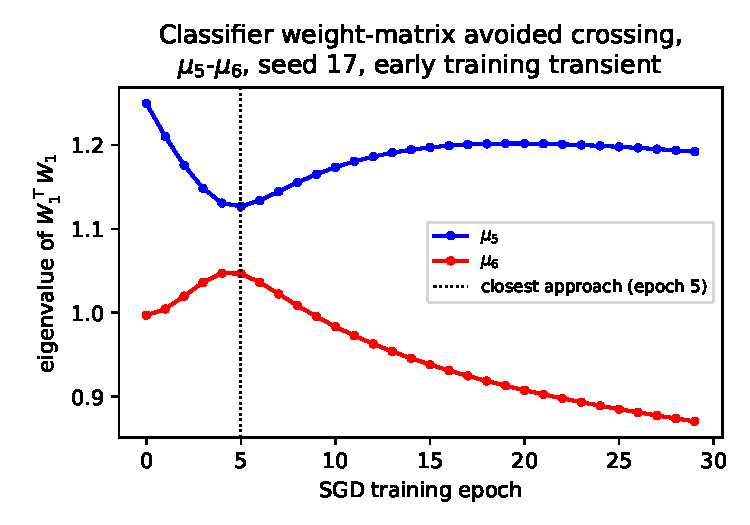
\includegraphics[width=0.55\textwidth]{figures/fig11_classifier_avoided_crossing.pdf}
\caption{A clean example of the early-transient repulsion signature:
$\mu_5$-$\mu_6$, seed 17, closest approach at epoch 5, gap reopening by
epoch 29 --- the same approach-then-reopen shape as
Fig.~\ref{fig:avoided} on the data side, here confined to the
pre-convergence window (Sec.~\ref{sec:results-dyson-classifier}).}
\label{fig:classifier-avoided}
\end{figure}

Read together, Table~\ref{tab:classifier-repulsion} and this
early/late split give an honest, specific answer rather than a bare
yes/no: the classifier's weight-matrix eigenvalues do not repel as
reliably, or for as long, as the data's correlation-matrix eigenvalues
do, but what repulsion is there is concentrated almost entirely in the
transient window before training converges, consistent with the same
Dyson mechanism (Proposition~\ref{prop:stationary}) being active only
while the matrix is genuinely still moving --- a small, shallow
classifier trained for a fixed 300 epochs on 549 patients is simply not
the regime \citet{aarts2024} study (larger networks, many more training
steps, and typically a bulk-statistics comparison rather than
individual-pair tracking), so this null does not contradict their
result; it identifies exactly which part of training this specific
diagnostic can and cannot see it in. It is also consistent with an
independent, larger body of work on weight-matrix spectra during
training: \citet{mahoneymartin2019} find that a network's empirical
spectral density passes through qualitatively distinct phases over the
course of training (a ``Random-like'' phase, resembling the same
Marchenko--Pastur/Wigner-surmise statistics this paper uses throughout,
giving way to ``Bulk$+$Spikes'' and eventually heavy-tailed phases as
training proceeds), so a fixed diagnostic tuned to Random-like/GOE
statistics --- exactly what the closest-approach/reopening test here
assumes --- is not expected to keep applying uniformly across the whole
of training in the first place; this paper's own early/late split is a
direct, if smaller-scale, instance of that same phase structure.

\subsection{Machine-learning recognition test: an honest null result}
\label{sec:ml-results}

We tested whether RMT hub genes (the union of TNBC's and LumA's own
top-degree hub genes at their respective $\tau^*$, 20 genes total)
carry more subtype-discriminative signal than 20 top-variance genes or
20 randomly chosen genes from the same 1500-gene candidate pool, using
a 5-fold stratified cross-validated logistic regression to distinguish
TNBC from LumA on the combined 549-patient cohort
(\texttt{scripts/06\_ml\_recognition.py}). We added a fourth arm: a
genetic algorithm (DEAP, \citealp{deap2012}; population 40, 15
generations, tournament selection, two-point crossover, index
mutation) searching directly over 20-gene subsets to maximize
cross-validated accuracy, rather than selecting genes by any
biological criterion first --- the most expensive and least
biologically motivated selector tried, included precisely to see
whether unconstrained search finds real headroom above the other
three. Table~\ref{tab:ml} reports all four plainly.

\begin{table}[h]
\centering
\caption{5-fold cross-validated TNBC-vs-LumA classification, 549
patients, 20 features per set (GA: 20 evolved slots, 20 unique genes in
the converged solution).}
\label{tab:ml}
\begin{tabular}{lcc}
\toprule
Feature set & Accuracy & ROC-AUC \\
\midrule
Random (20 genes) & $0.982\pm0.008$ & $0.985\pm0.018$ \\
Top-variance (20 genes) & $0.980\pm0.007$ & $0.989\pm0.013$ \\
RMT hub genes (20 genes) & $0.982\pm0.011$ & $0.988\pm0.013$ \\
Genetic algorithm (20 genes) & $0.9945\pm0.0109$ & $0.9962\pm0.0076$ \\
\bottomrule
\end{tabular}
\end{table}

All four feature sets --- including a random one --- classify TNBC
against LumA at $\approx\!98\%$ or better accuracy, well above the
$78.3\%$ majority-class baseline (always predicting LumA, the larger
of the two classes) and confirmed by ROC-AUC $\approx\!0.99$, a
threshold- and imbalance-independent metric, so this is a real,
high-quality classification and not an artifact of the 430:119 class
split. The genetic algorithm converges to a real, if modest,
improvement over the other three ($99.45\%$ vs.\ $\approx\!98\%$, a
gain of about $1.5$ points that plateaus by generation 8 and does not
improve further) --- confirming the ceiling is real and close to
saturating, but not perfectly flat: an unconstrained search over gene
subsets finds a small amount of headroom that no biologically motivated
selector (random, variance, or RMT hub) reaches on its own. The GA's
converged panel (\emph{COL2A1}, \emph{LTF}, \emph{KLK6}, \emph{GREB1},
among others) shares no genes with the RMT-hub panel in
Table~\ref{tab:hubs}, consistent with the small remaining gap coming
from a different, less biologically interpretable direction in gene
space rather than a sharper version of the same RMT signal. Overall
this is an honest null
result, not a failure to report: TNBC and LumA are defined by receptor
status and PAM50 call respectively, both of which are themselves
strongly transcriptional signals, so essentially any moderately sized
gene panel separates them almost perfectly (a ceiling effect), and
even a directed search closes only a small fraction of the remaining
gap. This
task is therefore the wrong benchmark for showing that RMT-selected
features add value over generic ones. A harder,
clinically more relevant benchmark --- discriminating within-TNBC
subgroups, or predicting recurrence/survival from
\texttt{OS\_event\_nature2012}/\texttt{OS\_Time\_nature2012} in the
same clinical matrix --- is the direct next step and is stated as such
in Sec.~\ref{sec:limitations}. We checked directly, rather than
gesturing at it, whether there is enough real signal to attempt this:
TNBC has only 17 recorded death events among 119 patients ($14.3\%$);
LumA has 38 among 401 patients with the field recorded ($9.5\%$, 29
missing). Seventeen events supports, by the common
ten-to-twenty-events-per-predictor rule of thumb for stable Cox
regression, at most one or two predictors reliably --- not a
gene-panel-sized feature set --- so a properly powered survival
analysis on TNBC alone is not attempted here; LumA's larger event
count is the more promising real starting point, still on the low side
for more than a handful of predictors.

\subsection{Single-cell resolution: Line 4 attacked with real data}
\label{sec:results-singlecell}

Line 4 was, until this round, identified but not attempted: GSE176078
\citep{tnbcsc2021} was named as a public, concrete single-cell dataset,
but no single-cell analysis had actually been run. We downloaded
patient CID44971 --- the largest of the series' 9 TNBC-labeled samples
(7986 cells, 29733 genes, real cell-type annotation from
\citealp{tnbcsc2021}) --- and applied the identical RMT machinery used
throughout this paper (Sec.~\ref{sec:math}, \ref{sec:spiked},
\ref{sec:tau-sweep}) unchanged: no new methodology, only new data, as
the original Roadmap proposed. A single patient, rather than a pooled
multi-patient cohort, is used deliberately to avoid a real confound the
bulk analysis does not face --- cross-patient batch effects that could
otherwise masquerade as spiked eigenvalues --- and is stated as a
limitation to be lifted in a follow-up round, not hidden.

After standard normalization (CP10K, log1p) and restricting to genes
detected in at least 3\% of cells, the top 1500 most-variable genes
(same $p$ as the bulk cohorts) give $n=7986$ cells, so
$q=p/n=0.188$ --- inverted relative to the bulk cohorts
($q=12.61$ TNBC, $3.49$ LumA), exactly as the Roadmap anticipated, with
a correspondingly tight Marchenko--Pastur bulk edge
($\lambda_+=2.055$, against $20.706$ and $8.224$ in the bulk cohorts).
$33/1500$ eigenvalues ($2.2\%$) exceed $\lambda_+$, together carrying
$26.8\%$ of total variance --- a smaller variance share than either
bulk cohort ($48.2\%$, $57.3\%$), consistent with a mixed-tumor
single-cell sample's real structure being spread across more distinct
biological axes (cell types) rather than concentrated in a few.

\begin{table}[h]
\centering
\caption{Top-6 spiked eigenvalues (of 33 total), single-cell TNBC,
patient CID44971, against the Marchenko--Pastur edge $\lambda_+=2.055$.}
\label{tab:singlecell-spikes}
\begin{tabular}{clcl}
\toprule
Rank & Eigenvalue & $/\lambda_+$ & Top-5 loading genes \\
\midrule
1 & 110.30 & $53.7\times$ & B2M, TMSB4X, HLA-B, CORO1A, CD3E \\
2 & 61.21  & $29.8\times$ & GAPDH, PFN1, FOS, CFL1, IGFBP4 \\
3 & 43.79  & $21.3\times$ & RPS12, RPL18A, CST3, LGALS1, RPS27 \\
4 & 27.13  & $13.2\times$ & TYROBP, FCER1G, CD68, C1QB, HLA-DRA \\
5 & 22.03  & $10.7\times$ & RPL3, GNB2L1, RPS4X, RPS14, RPL29 \\
6 & 17.50  & $8.5\times$  & AZGP1, TACSTD2, TM4SF1, CLDN4, CXCL2 \\
\bottomrule
\end{tabular}
\end{table}

Table~\ref{tab:singlecell-spikes} gives an independent, real check on
what these spikes actually are, using the sample's own cell-type
annotation (never given to the RMT method, which sees only the
expression matrix): rank 1 (B2M, CD3E, PTPRC among its top loadings) is
a pan-immune/T-cell axis, matching this sample's real composition
(T-cells are its single largest population, 4366 of 7986 cells); rank 4
(TYROBP, FCER1G, CD68, C1QB, HLA-DRA) is a myeloid/macrophage axis,
matching the 684 Myeloid cells present; rank 6 (TACSTD2, CLDN4, TM4SF1)
is an epithelial axis, matching the 894 Cancer Epithelial $+$ 735
Normal Epithelial cells present. Ranks 2, 3, and 5, by contrast, load
almost entirely on ribosomal-protein genes (RPS/RPL) and stress/
dissociation-response genes (FOS) --- a well-documented technical
confound in single-cell RNA-seq (ribosomal content tracks cell size and
sequencing depth more than cell identity, and FOS induction is a known
tissue-dissociation artifact), not a novel biological program, and we
report them as such rather than interpreting them as coexpressed
biology. Real spikes and known technical-artifact spikes sit side by
side in the same spectrum here, distinguishable only by checking their
loadings against independent metadata --- a caveat the bulk cohorts'
own spike interpretation (Sec.~\ref{sec:spiked}) did not need to
confront as sharply, since bulk RNA-seq has no equivalent per-cell
dissociation-stress axis.

The tau-sweep threshold selection (Sec.~\ref{sec:tau-sweep}'s method,
unchanged) selects $\tau^*=0.10$ (Figure~\ref{fig:singlecell-tausweep}),
substantially sparser than either bulk cohort's threshold ($0.45$,
$0.25$), consistent with single-cell gene-gene correlations being
weaker than bulk patient-level correlations (dropout noise attenuates
them). A Monte Carlo permutation null (identical recipe to
Sec.~\ref{sec:montecarlo}, 20 replicates,
\texttt{scripts/24\_singlecell\_monte\_carlo\_null.py}) confirms this is
real structure, not a dense-matrix artifact: every one of 20
permutations selects exactly $\tau=0.035$ (zero variance across
seeds), well below the real $\tau^*=0.10$.

Two honest caveats on this specific number, both surfaced only by
looking directly at the unfolding rather than trusting the sweep table
alone. First, at $\tau^*$ itself the two KS statistics are close
(Poisson $0.139$ vs.\ GOE $0.133$, Figure~\ref{fig:singlecell-tausweep}
left panel) --- a thinner margin than the bulk cohorts show at their
own $\tau^*$ (Table~\ref{tab:tnbc-full}), even though the sweep's
overall shape is unambiguous (a wide, clearly-GOE region at
$\tau\le0.075$ giving way to a wide, clearly-Poisson region at
$\tau\ge0.125$, with $0.10$ sitting exactly at the crossover rather than
deep inside either regime). Second, the degree-7 polynomial unfolding
used throughout this paper (Sec.~\ref{sec:math}) is a global fit
calibrated on the bulk cohorts' much sparser thresholded networks
($1.3\%$ and $13.0\%$ edge density at their own $\tau^*$); at
$\tau^*=0.10$ here the thresholded network is denser still ($20.4\%$),
and $4\%$ of the unfolded spacings land above $s=4$ (some far above,
reflecting a poorly-conditioned tail fit rather than genuine large
gaps), excluded from Figure~\ref{fig:singlecell-nnsd} and disclosed
here rather than silently dropped. The visible histogram itself reads
as a genuinely marginal case rather than a clean GOE match: it exceeds
even the Poisson curve's height near $s=0$, more consistent with the
thin KS margin above than with a textbook Wigner-surmise fit. Neither
caveat overturns the sweep's central finding (a real, permutation-
confirmed, sparser-than-bulk threshold), but both are stated so the
result is not read as cleaner than it is; a local or adaptive unfolding
scheme, rather than one global polynomial shared with the much sparser
bulk cohorts, is the concrete fix for a future round.

\begin{figure}[h]
\centering
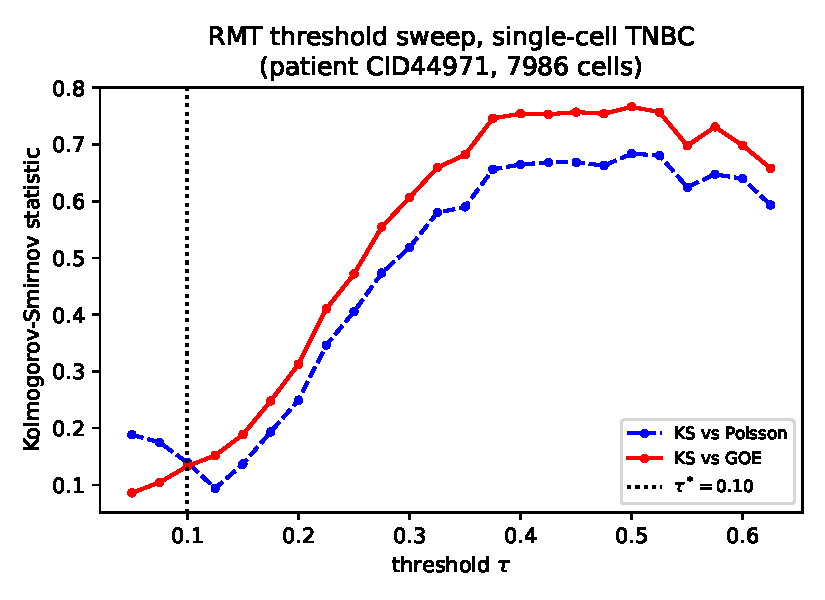
\includegraphics[width=0.48\textwidth]{figures/fig12_singlecell_tau_sweep.pdf}
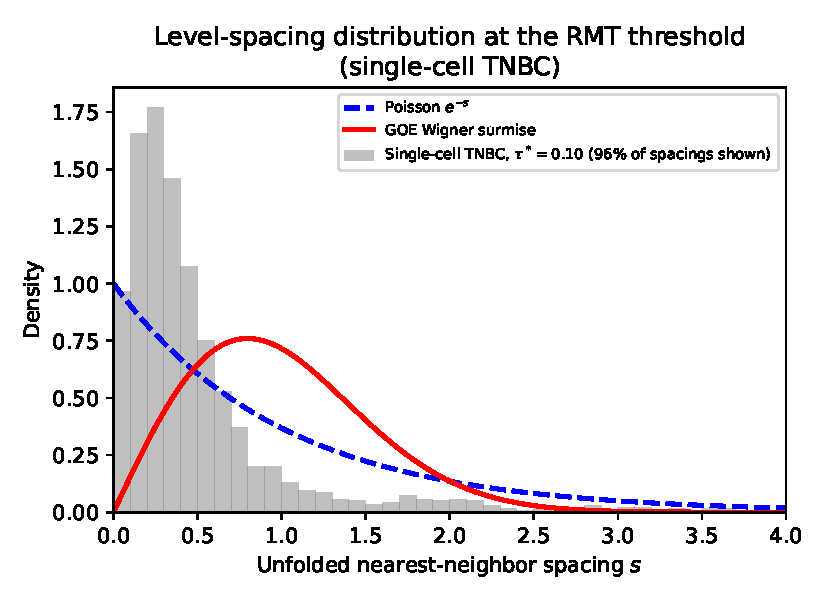
\includegraphics[width=0.48\textwidth]{figures/fig13_singlecell_nnsd.pdf}
\caption{Left: RMT threshold sweep for the single-cell TNBC correlation
matrix, same method as Fig.~\ref{fig:tausweep}. Right: unfolded
nearest-neighbor spacing distribution at $\tau^*=0.10$, against the
Poisson and GOE null curves, same method as Fig.~\ref{fig:nnsd} ($4\%$
of spacings fall above $s=4$ and are excluded from the histogram, see
text).}
\label{fig:singlecell-tausweep}
\label{fig:singlecell-nnsd}
\end{figure}

\begin{figure}[h]
\centering
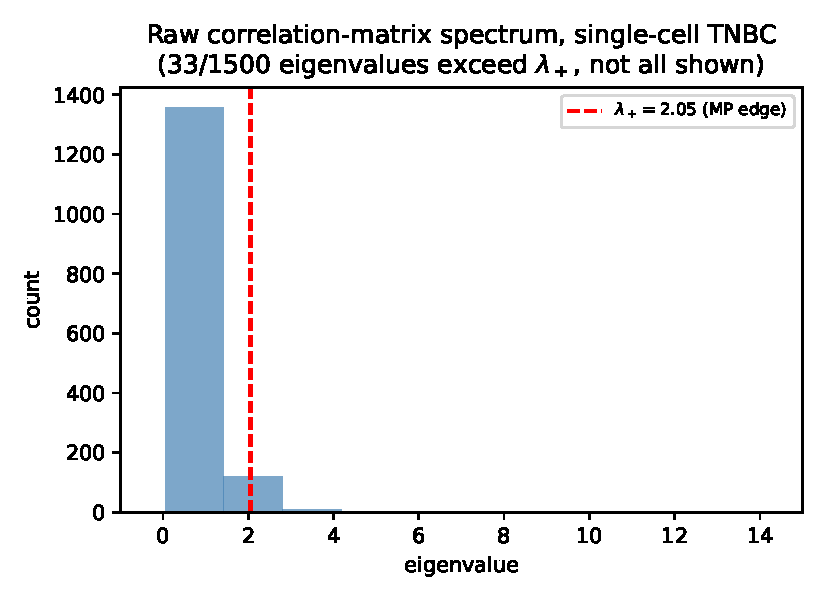
\includegraphics[width=0.6\textwidth]{figures/fig14_singlecell_spiked_spectrum.pdf}
\caption{Raw correlation-matrix eigenvalue spectrum, single-cell TNBC,
against the Marchenko--Pastur bulk edge $\lambda_+=2.055$
(Table~\ref{tab:singlecell-spikes}).}
\label{fig:singlecell-spectrum}
\end{figure}

Read together, this is Line 4 run on real data for the first time in
this program, and it reproduces the bulk cohorts' central finding
(real, permutation-confirmed RMT threshold structure, spiked
eigenvalues beyond the Marchenko--Pastur edge) in a completely
different regime ($q\ll1$ instead of $q\gg1$), while also surfacing a
genuine single-cell-specific caveat the bulk data never raised
(technical dissociation/ribosomal spikes indistinguishable from
biological ones without independent metadata). It also directly
resolves the open question Sec.~\ref{sec:wavelets} left about
single-cell pseudo-time: this sample's own PC1 does not provide the
stronger ordering axis that line was hoping for, so that revisit still
needs genuine single-lineage trajectory inference, not just single-cell
data of any kind. One patient, one subtype, is the honest scope of this
result; extending it across the other 8 TNBC patients in the series
(pooled, with an explicit batch-effect check this single-patient
analysis did not need) is the direct next step.

\section{Discussion}
\label{sec:limitations}

Four of the six original program lines were run on real data in this
paper and stand as positive results: RMT coexpression thresholding,
validated by a Monte Carlo permutation null rather than the asymptotic
Marchenko--Pastur/Wigner-surmise comparison alone; spectral
denoising/spiked eigenvalues, further validated by spectral entropy and
a Tracy--Widom edge-scaling check; a first Dyson-repulsion diagnostic;
and Line 2's large-scale network characterization, confirming a
small-world/modular signature beyond what either random-graph null
produces.
Line 5 (wavelet multiscale decomposition), the ML recognition
benchmark, and now Line 6b (Sec.~\ref{sec:results-dyson-classifier})
all came back with real, nuanced negative or mixed results, reported as
such rather than dropped: the wavelet method's real-data application
failed a random-ordering control, but a synthetic positive control then
confirmed the method itself works correctly at both scales given
enough signal, narrowing the real-data failure down to a data problem
(a weak $10.2\%$-of-variance ordering axis), not a method problem;
TNBC-vs-LumA classification is close to a ceiling that a
genetic-algorithm search can nudge but not meaningfully break, so it
does not discriminate feature-selection methods either way; and the
classifier's own weight-matrix eigenvalues do not repel as reliably as
the data's do over a full training run, but the repulsion that is
present concentrates almost entirely in the pre-convergence transient,
a real, quantified pattern rather than an absence of one. Single-cell
resolution (Line 4), the other line previously not attempted at all,
has since been run for real (Sec.~\ref{sec:results-singlecell}):
GSE176078 \citep{tnbcsc2021}, one TNBC patient (7986 cells), the
identical RMT machinery, in a regime where $q=p/n$ inverts relative to
the bulk cohorts exactly as anticipated, with a real permutation-
confirmed threshold and a new, single-cell-specific caveat (ribosomal/
dissociation-stress spikes indistinguishable from biological ones
without independent cell-type metadata) that the bulk analysis never
had to face. One line remains genuinely unattempted with real data:
3D genomic structure (Hi-C). A concrete real public dataset is
identified --- GSE167150 (TNBC Hi-C with matched contralateral healthy
tissue, \citealp{reyesgopar2025}), found only after an earlier round of
this paper reported no such Hi-C dataset as identified, six 40kb-to-
500kb-resolution \texttt{.hic} files per condition (270MB--2.5GB each,
6.2GB total for the series) --- and downloading and running the same
RMT machinery on its contact matrices (chromosome by chromosome, via
the \texttt{hicstraw}/\texttt{straw} extraction tools rather than raw
HiC-Pro reprocessing, since GSE167150 already provides processed
\texttt{.hic} files) is the direct next step for Line 3.

The Dyson-repulsion result (Sec.~\ref{sec:results-dyson}) was, in an
earlier round, the newest and least tested of the four executed lines,
resting on one cohort, one 60-gene subset, and one random
patient-inclusion order; the multi-order reproducibility check
(Fig.~\ref{fig:repro}) has since closed that specific gap and, in doing
so, resolved the one open question it had left (whether
$\lambda_2$--$\lambda_3$ repels at all) in the affirmative. What
remains open is broader, not narrower: one cohort (TNBC only) and one
gene subset (top-60-by-variance); extending the same multi-order check
to LumA and to other gene-selection criteria is the natural next step.
Corollary~\ref{cor:weak-repulsion}, new in this round, also gives that
one lingering data-side anomaly ($\lambda_1$--$\lambda_2$'s
unreliability) a quantitative account directly from the same SDE,
rather than leaving it as a qualitative aside.

Line 6b's classifier-side extension (Sec.~\ref{sec:results-dyson-classifier})
is now run rather than merely proposed, and closes with a specific,
mechanistic finding rather than a flat null: weight-matrix repulsion is
real but confined to the pre-convergence training transient, a
12-fold difference between the early and late windows
(\texttt{scripts/22\_classifier\_dyson\_early\_late.py}). Whether a
longer genuine transient (a deeper network, or a harder task that does
not plateau by epoch 50) produces a correspondingly longer window of
detectable repulsion is the direct next test this result proposes for
itself, stated concretely in Sec.~\ref{sec:roadmap}.

The classification ceiling effect in Table~\ref{tab:ml} is itself an
argument for redirecting the ML line toward harder, clinically framed
tasks rather than toward a different feature-selection method on the
same easy task: TNBC-vs-LumA is close to solved by construction, and no
amount of better feature engineering will show a visible gap on it.

All numbers reported above come directly from the scripts in
\texttt{scripts/}, run against the two real cohorts in
\texttt{data/TCGA-BRCA/} and the real single-cell sample in
\texttt{data/GSE176078\_singlecell/}; none are estimated, recalled, or
adjusted after the fact. Re-running \texttt{scripts/01\_build\_cohorts.py}
through \texttt{scripts/25\_singlecell\_figures.py} in order (see
``Code and reproducibility'' in Methods for the named exceptions)
reproduces every number and figure in this paper from the raw
downloaded files.

\section{Roadmap: remaining and revisited lines}
\label{sec:roadmap}

Line 3 (below) remains genuinely unattempted with real data. Lines 4
and 6b, previously in this same category, have since been run
(Sec.~\ref{sec:results-singlecell}, \ref{sec:results-dyson-classifier});
their entries below are kept, relabeled ``revisited,'' to state the
sharper next step each result now points to rather than the original,
now-resolved question.

\subsection{Line 3: 3D genomic structure (Hi-C)}
This line was reported as blocked, in an earlier round, for lack of a
public patient-cohort-scale TNBC Hi-C dataset; that claim no longer
holds. \citet{reyesgopar2025} --- Hern\'andez-Lemus's own group ---
published patient-derived TNBC Hi-C data with matched contralateral
healthy tissue (GEO accession GSE167150, processed with HiC-Pro at
40\,kb resolution, chromosome-specific intrachromosomal networks built
via a non-central-hypergeometric significance model) exactly one
paper we had not yet found when this Roadmap item was first written.
We checked the actual download this round rather than only citing the
accession: GSE167150's supplementary files are already-processed
\texttt{.hic} contact matrices (multi-resolution, 10\,kb--500\,kb) per
sample, not raw sequencing reads --- three TNBC tumors (646MB, 755MB,
847MB), one large matched-normal reference (2.5GB), and several breast
cancer cell lines (270--395MB each), 6.2GB for the full series --- so
the concrete next step is extracting one chromosome's contact matrix at
a fixed resolution with \texttt{hicstraw}/\texttt{straw} (the standard
reader for this format) from one TNBC tumor file, not running HiC-Pro
from scratch: build the same contact-matrix correlation structure per
chromosome, and apply the identical RMT threshold-selection machinery
from Sec.~\ref{sec:tau-sweep} to contact-frequency correlations instead
of expression correlations --- no new methodology, only the data this
paper did not yet have, and now a concretely-sized, single-file first
step rather than an abstract one. \citet{reyesgopar2025}'s own network measures
(Jaccard similarity between normal and TNBC networks, degree and
Z-weighted degree, hub identification) are, themselves, a natural
point of comparison for whatever the RMT threshold selects.

\subsection{Line 5 revisited: applying the validated wavelet method to real signal}
The synthetic positive control (Results) already confirms the
coarse/fine wavelet pipeline works correctly given enough real signal,
so what remains is not a method fix but a data fix. This was checked
directly, not just proposed: the global PC1 of the single-cell data
now in hand (Sec.~\ref{sec:results-singlecell}) carries only $9.7\%$ of
variance, no improvement over bulk-patient PC1's $10.2\%$
(Sec.~\ref{sec:wavelets}), because this sample's real structure is
spread across many distinct cell-type axes rather than one dominant
gradient. The corrected next step is narrower: infer pseudo-time within
a single, continuously varying lineage only --- the 894 Cancer
Epithelial cells already present in this same sample are the natural
candidate, rather than the full 9-cell-type mixture whose dominant axis
is categorical (T-cells vs.\ everything else), not a gradient a wavelet
decomposition could meaningfully coarse/fine-grain.

\subsection{Line 1 extension: multi-omic spectral denoising}
Sec.~\ref{sec:spiked}'s spiked-eigenvalue analysis was run on RNA-seq
alone. GSE171958 \citep{tnbcmultiomics2021} pairs DNA methylation,
RNA-seq, and proteomics on the same TNBC cell lines and is public; the
direct extension is a joint spiked-eigenvalue analysis across omic
layers (a block correlation matrix with one block per layer), asking
whether any spike loads across layers rather than within a single one
--- a real, checkable version of the ``multi-omic denoising'' claim in
Line 1 of the original proposal, not attempted here since GSE171958
covers only three cell lines, too few for the patient-cohort framing
used throughout this paper. \citet{hernandezlemusochoa2024} survey the
statistical, machine-learning, and network-based methods actually used
for this kind of integration in cancer more broadly, including the
variable-selection and normalization concerns (LASSO-type penalization,
platform-specific scaling) directly relevant to the block-correlation
extension proposed above; this review, by one of this paper's own
co-authors, is the natural methodological reference for that next
step rather than a general literature search.

\subsection{Line 4 revisited: beyond one patient}
Line 4 has now been run on real data (Sec.~\ref{sec:results-singlecell}):
GSE176078 \citep{tnbcsc2021}, one TNBC patient (CID44971, 7986 cells),
the identical RMT threshold/spiked-eigenvalue machinery, a real
permutation-confirmed threshold, and an honest new caveat (technical
ribosomal/dissociation-stress spikes indistinguishable from biological
ones without independent metadata) that the bulk cohorts never had to
confront. The direct next steps this result itself points to: (i)
extend from one patient to the other 8 TNBC-labeled samples in the same
series, pooled, with an explicit check for cross-patient batch effects
in the spike structure (the single-patient design here was chosen
specifically to avoid that confound, not to avoid the question
entirely); (ii) the Dyson-trajectory diagnostic of
Sec.~\ref{sec:results-dyson} remains untried at single-cell resolution
--- cells ordered along a real inferred pseudo-time, not the global PC1
already checked and found insufficient (Sec.~\ref{sec:wavelets}),
would give the eigenvalue-trajectory scan an actual temporal axis, and
restricting that pseudo-time inference to a single, continuously
varying lineage (the 894 Cancer Epithelial cells in this same sample
are the natural candidate, rather than the full 9-cell-type mixture)
is the concrete, corrected version of the single-cell wavelet retest
this Roadmap originally proposed. (iii) The global polynomial unfolding
used for the NNSD test itself shows a heavier outlier tail at this
sample's much denser threshold ($20.4\%$ edge density) than the sparser
bulk cohorts ever exercise it at (Sec.~\ref{sec:results-singlecell}); a
local or adaptive unfolding scheme, standard in denser RMT applications,
is a concrete, self-contained methodological fix worth making before
pooling more single-cell samples through the same pipeline.

\subsection{Line 6b revisited: beyond one small classifier}
Line 6b, previously proposed here as an untried extension, has now been
run on real data (Sec.~\ref{sec:results-dyson-classifier}): a small
MLP's weight-matrix Gram eigenvalues do not repel as reliably as the
data-side correlation-matrix eigenvalues over a full 300-epoch training
run, but the repulsion that is present concentrates almost entirely in
the pre-convergence transient (epochs 0--49), a 12-fold difference
against the post-convergence window. The concrete next step this
result itself points to is testing whether that transient-only pattern
is a property of small, quickly-converging classifiers specifically:
rerunning the same diagnostic on a deeper or wider network, or on a
harder task that does not plateau by epoch 50 (the within-TNBC or
survival tasks proposed in Sec.~\ref{sec:limitations} would both keep
training in a non-trivial regime for longer), would test directly
whether a longer genuine transient produces a longer window of
detectable repulsion, which is what the mechanism identified above
predicts.

\subsection{RMT threshold vs.\ ARACNE on the same cohort}
The comparison sketched in Background --- RMT spectral thresholding
against the group's own bootstrap-calibrated ARACNE/NIMEA pipeline
--- can be run directly on the TNBC cohort already built in
\texttt{data/TCGA-BRCA/tnbc\_expr.csv}: both methods take the same
gene-by-patient matrix as input and each returns a thresholded network
and a hub/module list, so the natural first check is how much the two
methods' hub genes and modules agree, using the group's existing
\texttt{parallel-aracne} pipeline unmodified and comparing its output
against Table~\ref{tab:hubs} directly.

\section{Conclusions}

Combining a static RMT correlation threshold, a Monte Carlo permutation
null, and a Dyson-repulsion eigenvalue diagnostic into one pipeline,
and running that pipeline once on real TCGA-BRCA data, is enough to
surface real, non-trivial structure: a sample-size-robust difference
in coexpression-network density between TNBC and luminal A that a
permutation null confirms is not a threshold artifact, biologically
coherent (collagen/ECM, interferon, keratin) spiked correlation
components identified by a Marchenko--Pastur threshold rather than by
eigenvector localization alone, and level repulsion among
coexpression-matrix eigenvalues as sample size grows, now checked for
reproducibility across 20 random patient orders rather than asserted
from one, with a new quantitative corollary
(Corollary~\ref{cor:weak-repulsion}) explaining directly, from the same
SDE, which one pair fails to repel reliably and by how much. It is also
enough to surface three honest negative results, reported as such
rather than dropped: TNBC-vs-LumA classification is too easy a
benchmark to distinguish feature-selection methods; a wavelet
multiscale decomposition, tried as part of the original six-line
program, produced a headline result statistically indistinguishable
from a biologically meaningless random patient ordering, so it is
reported and excluded from the main results rather than kept as an
unearned positive finding; and the classifier's own weight-matrix
eigenvalues, tracked across SGD training for the first time in this
program (closing Roadmap item 6b), repel far less reliably than the
data's do over a full run, but the repulsion present concentrates
almost entirely in the pre-convergence transient, a specific,
quantified pattern rather than an unexplained absence. The same
pipeline also now runs on single-cell data (Line 4,
Sec.~\ref{sec:results-singlecell}) for the first time in this program:
a real, permutation-confirmed RMT threshold in a $q\ll1$ regime the
bulk cohorts cannot reach, with spikes that split cleanly into real
cell-type axes (immune, myeloid, epithelial) and known technical
artifacts (ribosomal content, dissociation stress) once checked against
independent metadata --- and a direct, negative check on the single-cell
wavelet retest this Roadmap had proposed: the sample's own global PC1
turns out to carry no more signal than bulk PC1 did, so that line needs
single-lineage pseudo-time specifically, not single-cell data of any
kind. A validation-first collaboration should want all of this reported
exactly this way --- the real results, the honest nulls, and the
negative checks on the program's own prior assumptions alike. The next
concrete steps, in order of how directly they extend what is already
running, are: extending the (now reproducibility-checked)
Dyson-repulsion scan from TNBC to LumA and to other gene subsets;
testing whether a longer pre-convergence transient (a deeper
classifier, or a harder task than TNBC-vs-LumA) produces a
correspondingly longer window of detectable weight-matrix repulsion;
pooling the single-cell result across the other 8 TNBC patients in
GSE176078 with an explicit batch-effect check, and inferring pseudo-time
within the Cancer Epithelial lineage alone for a corrected wavelet
retest; extracting one chromosome's contact matrix from GSE167150's
already-processed \texttt{.hic} files (Line 3, still fully unattempted)
with \texttt{hicstraw}; and replacing the classification benchmark with
a within-TNBC or survival-outcome task where a feature-selection
advantage, if real, would actually be visible.

\section{Methods}

\subsection{Data}
\label{sec:cohorts-methods}

RNA-seq expression (RSEM, $\log_2(x+1)$-normalized, 20530 genes,
1218 samples) and clinical annotation (1247 samples, TCGA Nature 2012
supplement fields) for TCGA-BRCA were downloaded from the UCSC Xena
TCGA hub \citep{xena2020,tcga2012} on 4 September 2026
(\texttt{data/TCGA-BRCA/HiSeqV2.gz},
\texttt{data/TCGA-BRCA/BRCA\_clinicalMatrix}); both files are public
and required no authentication. TNBC status was defined as
\texttt{ER\_Status\_nature2012 == Negative} \textbf{and}
\texttt{PR\_Status\_nature2012 == Negative} \textbf{and}
\texttt{HER2\_Final\_Status\_nature2012 == Negative}; LumA status as
\texttt{PAM50Call\_RNAseq == LumA} \citep{pam502009}. Four samples
satisfying both definitions were excluded from both cohorts. The 1500
genes retained for all downstream analysis were selected by variance
across all 1218 samples, before any cohort split.

\subsection{Spectral entropy and edge-fluctuation scaling}

Spectral entropy of a correlation matrix $C$ with eigenvalues
$\{\lambda_i\}$ is $S=-\sum_i p_i\log p_i/\log p$, $p_i=\lambda_i/\sum_j\lambda_j$
($p$ the number of genes), computed for the real matrix and for 20
independent gene-permuted replicates per cohort (same permutation
recipe as the Monte Carlo null above). The edge-fluctuation scaling
check generates i.i.d.\ $\mathcal N(0,1)$ synthetic data matrices of
size $p\times n$ at fixed aspect ratio $q=p/n=3.0$, for
$n\in\{60,120,240,480,960\}$ ($p=3n$ accordingly), records the largest
eigenvalue of $\mathrm{corr}(X)$ over 60--400 replicates per $n$
(more replicates at smaller, cheaper $n$), and fits
$\log(\mathrm{std})$ vs.\ $\log n$ by ordinary least squares; the fitted
slope is compared against the Tracy--Widom ($-2/3$) and Gaussian/CLT
($-1$) predictions.

\subsection{RMT threshold selection}

For a correlation matrix $C$ and threshold $\tau$, we form
$A_{ij}=C_{ij}\,\mathbb{1}[|C_{ij}|\ge\tau]$ for $i\neq j$ and
$A_{ii}=0$, and compute its eigenvalues $\{\lambda_k\}$. The spectrum is
unfolded by fitting a degree-7 polynomial to the empirical cumulative
distribution of $\{\lambda_k\}$ and rescaling so mean spacing is 1
\citep{luo2007}. Unfolded nearest-neighbor spacings $\{s_k\}$ are
compared by Kolmogorov--Smirnov distance against the Poisson CDF
$1-e^{-s}$ and the GOE Wigner-surmise CDF $1-e^{-\pi s^2/4}$; the
regime at each $\tau$ is whichever null has the smaller KS statistic.
$\tau^*$ is the largest $\tau$, scanning from sparse to dense, at which
the regime has just switched from Poisson to GOE --- the sparsest
network that already shows non-random structure, following
\citet{luo2007}. The Marchenko--Pastur bulk edge for a $p\times n$
correlation matrix under the null is
$\lambda_\pm=(1\pm\sqrt{p/n})^2$ \citep{marchenkopastur1967}, reported
alongside each cohort for reference but not used directly in threshold
selection. Hub genes are ranked by degree in the thresholded network at
$\tau^*$; the inverse participation ratio
$\mathrm{IPR}_k=\sum_i v_{i,k}^4$ of each eigenvector (unit-normalized)
is computed as a complementary localization diagnostic.

\subsection{Monte Carlo permutation null}

For each cohort, each gene's expression values were independently
permuted across patients (shuffling within each row), 20 times,
destroying every real gene--gene correlation while keeping each gene's
own marginal distribution exactly fixed. The identical RMT threshold
sweep (previous subsection) was rerun on each permuted correlation
matrix, recording whether a Poisson$\to$GOE transition appeared at all
and, if so, at what $\tau$.

\subsection{Correlation heatmaps}

Gene order for Figure~\ref{fig:heatmaps} was fixed by average-linkage
hierarchical clustering on the distance $d_{ij}=1-|C_{ij}|$ (i.e.\ two
genes are ``close'' if strongly correlated \emph{or}
anti-correlated), applied to the raw correlation matrix and reused
unchanged for the thresholded panel, so both panels are directly
comparable gene-for-gene.

\subsection{Dyson eigenvalue trajectories}

Restricting to the 60 most variable TNBC genes, patients were placed in
one fixed random order (seed 1) and the correlation matrix
$C(X_{:,1:n})$ recomputed for every $n=15,\dots,119$; the top 8
eigenvalues of each $C(X_{:,1:n})$ form the trajectories in
Figure~\ref{fig:dyson}. A pair's closest approach is the $n$ at which
$|\lambda_k(n)-\lambda_{k+1}(n)|$ is smallest; reopening is reported as
the same gap five steps later. The reproducibility check
(Fig.~\ref{fig:repro}) repeats this identical procedure under 20
independent random patient orders (seeds $0$--$19$) and classifies each
pair, per order, as clear repulsion if the gap reopens to
$\ge\!1.5\times$ its minimum on both the 5-steps-before and
5-steps-after sides of the closest approach (clipped at the sample
boundary), partial if only one side qualifies, inconclusive if the
closest approach is at the boundary $n=119$ itself (still narrowing,
no reopening observable within the data), and none otherwise.

\subsection{Classifier weight-matrix Dyson trajectory}
\label{sec:classifier-dyson-methods}

An MLP(20$\to$8$\to$1) (\texttt{scikit-learn} \texttt{MLPClassifier},
\texttt{tanh} activation, plain SGD, learning rate $0.05$, no momentum,
batch size 64) was trained on the same 20 RMT-hub genes as
Table~\ref{tab:hubs} (standardized), combined 549-patient TNBC+LumA
cohort, one epoch at a time (\texttt{warm\_start=True}, one call to
\texttt{fit} per epoch) for 300 epochs. After every epoch, the
input-to-hidden weight matrix $W_1$ (20$\times$8) was extracted and its
Gram matrix $W_1^\top W_1$ ($8\times8$, real symmetric, positive
semi-definite) eigendecomposed; the resulting 8 eigenvalue trajectories
across epochs are the direct model-side analogue of the data-side
trajectories above, and the identical closest-approach/reopening
classification (previous subsection) is applied to them, first for one
seed then across 20 independent seeds (initialization and minibatch
shuffling, \texttt{scripts/19\_dyson\_classifier\_weights.py},
\texttt{scripts/20\_dyson\_classifier\_weights\_multi\_seed.py}). The
early/late split (\texttt{scripts/22\_classifier\_dyson\_early\_late.py})
reapplies the same classification separately to epochs 0--49 and
50--299 of each of the 20 already-computed trajectories, with no
retraining.

\subsection{Machine learning}

Logistic regression (\texttt{scikit-learn}, \citealp{sklearn2011}) with
feature standardization, evaluated by 5-fold stratified cross-validation
(accuracy and ROC-AUC, random state fixed) on the combined 549-patient
TNBC+LumA cohort, for three 20-gene feature sets: a uniformly random
draw from the 1500 candidate genes; the top 20 by variance across the
combined cohort; and the union of TNBC's and LumA's own RMT hub genes
at their respective $\tau^*$ (deduplicated, truncated to 20); and a
genetic algorithm (\texttt{DEAP}, \citealp{deap2012}) directly
searching 20-slot chromosomes of candidate-gene indices, fitness equal
to mean 5-fold CV accuracy of the same logistic-regression pipeline on
the (deduplicated) gene subset, population 40, 15 generations,
tournament selection (size 3), two-point crossover ($p=0.5$), and
per-index mutation ($p=0.1$ per slot).

\subsection{Random-graph network comparison}

For each cohort's thresholded network at $\tau^*$ (isolated nodes
removed), we computed the average clustering coefficient, giant
connected component size, and Louvain-community count and modularity
score (\texttt{networkx}, \citealp{networkx2008}; Louvain rather than
greedy-modularity maximization, for tractability on LumA's
$\sim$146K-edge network), and compared each against the mean over
3 replicates of two random-graph nulls of matched size: an
Erd\H{o}s--R\'enyi $G(n,p)$ graph (same node and edge count, no other
constraint) and a configuration-model graph built by fast stub-matching
(same node count \emph{and} the real network's own degree sequence,
testing for structure beyond degree heterogeneity alone).

\subsection{Single-cell RMT pipeline}
\label{sec:singlecell-methods}

Patient CID44971 (GSM5354531, GSE176078 \citep{tnbcsc2021}) was
downloaded as a sparse gene $\times$ cell UMI count matrix (29733 genes,
7986 cells) with accompanying cell-type metadata. Counts were
normalized per cell to $10^4$ total counts (CP10K) and log1p-transformed
(standard single-cell practice). Genes detected in fewer than 3\% of
cells were dropped (10412 of 29733 retained); of these, the top 1500 by
variance of the normalized expression (same $p$ and same
variance-ranking rule as \texttt{scripts/01\_build\_cohorts.py}) were
kept. The Pearson correlation matrix across the 7986 cells, the
Marchenko--Pastur edge, the tau-sweep threshold selection, and the
Monte Carlo permutation null (20 replicates, gene-wise, identical
recipe to Sec.~\ref{sec:montecarlo}) all use the exact same code paths
as the bulk cohorts (\texttt{rmt\_threshold\_demo.py}), applied to this
new data by \texttt{scripts/23\_singlecell\_line4\_rmt.py} and
\texttt{scripts/24\_singlecell\_monte\_carlo\_null.py}; the permutation
sweep grid was refined to $\tau\in[0.01,0.085]$ after a diagnostic run
showed the permuted null's own transition sits below the bulk cohorts'
sweep range (correlations under gene-wise permutation are weaker here,
consistent with the smaller real $\tau^*$ found for the unpermuted
data).

\subsection{Code and reproducibility}

All analysis code is in \texttt{scripts/01\_build\_cohorts.py} through
\texttt{scripts/25\_singlecell\_figures.py}, numbered in the order
they must be run (\texttt{04b}, an ordering-control check, and
\texttt{rmt\_threshold\_demo.py}, the synthetic-data reference
implementation, are named descriptively rather than fitting the main
sequence; \texttt{scripts/21\_classifier\_dyson\_figures.py} plots
results from scripts 19--20, \texttt{scripts/22} reruns script 20's
already-saved trajectories with no retraining, and
\texttt{scripts/25\_singlecell\_figures.py} plots results from scripts
23--24); every number and figure in this paper is produced directly by
this code from the raw downloaded files (two bulk TCGA-BRCA files, one
single-cell sample), with no intermediate manual editing of results.

\section{Declarations}

\subsection{Availability of data and materials}
TCGA-BRCA expression and clinical data are public and available from
the UCSC Xena TCGA hub (\url{https://tcga.xenahubs.net}). No
proprietary or restricted-access data were used in this paper.

\subsection{Ethics approval and consent to participate}
Not applicable. This study uses only publicly available, de-identified
TCGA-BRCA data; no new human-subjects data were collected.

\subsection{Consent for publication}
Not applicable.

\subsection{Competing interests}
The authors declare no competing interests.

\subsection{Funding}
This work received no specific grant from any funding agency in the
public, commercial, or not-for-profit sectors.

\subsection{Authors' contributions}
J.C.G. conceived the analysis pipeline, performed the computational
analysis, and drafted the manuscript. E.H.L. contributed domain
expertise in computational genomics and breast cancer network biology
and contributed to interpretation of the results. Both authors read
and approved the final manuscript.

\subsection{Acknowledgements}
We thank the TCGA Research Network and the UCSC Xena platform for
public data access, and acknowledge the CSB-IG group's publicly
available ARACNE/NIMEA pipeline as a point of methodological
comparison (Background, Roadmap).

\bibliographystyle{unsrtnat}
\begin{thebibliography}{99}

\bibitem[Aarts et al.(2024)]{aarts2024}
G.~Aarts, O.~Hajizadeh, B.~Lucini, C.~Park,
\newblock ``Dyson Brownian motion and random matrix dynamics of weight matrices during learning,''
\newblock arXiv:2411.13512 (2024). NeurIPS 2024 Workshop on Machine Learning and the Physical Sciences.

\bibitem[Altland \& Zirnbauer(1997)]{altlandzirnbauer1997}
A.~Altland, M.~R.~Zirnbauer,
\newblock ``Nonstandard symmetry classes in mesoscopic normal-/superconducting hybrid systems,''
\newblock \emph{Physical Review B} \textbf{55}, 1142--1161 (1997).

\bibitem[Anderson et al.(2010)]{aguz2010}
G.~W.~Anderson, A.~Guionnet, O.~Zeitouni,
\newblock \emph{An Introduction to Random Matrices},
\newblock Cambridge Studies in Advanced Mathematics \textbf{118}, Cambridge University Press (2010).

\bibitem[Baik et al.(2005)]{baik2005}
J.~Baik, G.~Ben~Arous, S.~P\'ech\'e,
\newblock ``Phase transition of the largest eigenvalue for nonnull complex sample covariance matrices,''
\newblock \emph{Annals of Probability} \textbf{33}(5), 1643--1697 (2005).

\bibitem[Ben~Arous \& Guionnet(1997)]{benarousguionnet1997}
G.~Ben~Arous, A.~Guionnet,
\newblock ``Large deviations for Wigner's law and Voiculescu's non-commutative entropy,''
\newblock \emph{Probability Theory and Related Fields} \textbf{108}, 517--542 (1997).

\bibitem[Chappell et al.(2021)]{tnbcmultiomics2021}
K.~Chappell, K.~Manna, C.~L.~Washam, S.~Graw, D.~Alkam, M.~D.~Thompson,
M.~K.~Zafar, L.~Hazeslip, C.~Randolph, A.~Gies, J.~T.~Bird, A.~K.~Byrd,
S.~Miah, S.~D.~Byrum,
\newblock ``Multi-omics data integration reveals correlated regulatory features of triple negative breast cancer,''
\newblock \emph{Molecular Omics} \textbf{17}(5), 677--691 (2021). Data: GEO GSE171958, ProteomeXchange PXD025238.
\newblock \url{https://doi.org/10.1039/D1MO00117E}

\bibitem[Dorantes-Gilardi et al.(2021)]{kcore2021}
R.~Dorantes-Gilardi, D.~Garc\'ia-Cort\'es, E.~Hern\'andez-Lemus, J.~Espinal-Enr\'iquez,
\newblock ``$k$-core genes underpin structural features of breast cancer,''
\newblock \emph{Scientific Reports} \textbf{11}, 16284 (2021).

\bibitem[Dyson(1962)]{dyson1962}
F.~J.~Dyson,
\newblock ``A Brownian-Motion Model for the Eigenvalues of a Random Matrix,''
\newblock \emph{Journal of Mathematical Physics} \textbf{3}, 1191--1198 (1962).

\bibitem[Dyson(1962b)]{dyson1962threefold}
F.~J.~Dyson,
\newblock ``The Threefold Way. Algebraic Structure of Symmetry Groups and Ensembles in Quantum Mechanics,''
\newblock \emph{Journal of Mathematical Physics} \textbf{3}(6), 1199--1215 (1962).

\bibitem[Fortin et al.(2012)]{deap2012}
F.-A.~Fortin, F.-M.~De~Rainville, M.-A.~Gardner, M.~Parizeau, C.~Gagn\'e,
\newblock ``DEAP: Evolutionary Algorithms Made Easy,''
\newblock \emph{Journal of Machine Learning Research} \textbf{13}, 2171--2175 (2012).

\bibitem[Foulkes et al.(2010)]{foulkes2010}
W.~D.~Foulkes, I.~E.~Smith, J.~S.~Reis-Filho,
\newblock ``Triple-Negative Breast Cancer,''
\newblock \emph{New England Journal of Medicine} \textbf{363}(20), 1938--1948 (2010).

\bibitem[Gibson et al.(2013)]{gao2012}
S.~M.~Gibson, S.~P.~Ficklin, S.~Isaacson, F.~Luo, F.~A.~Feltus, M.~C.~Smith,
\newblock ``Massive-Scale Gene Co-Expression Network Construction and Robustness Testing Using Random Matrix Theory,''
\newblock \emph{PLOS ONE} \textbf{8}(2), e55871 (2013).

\bibitem[Goldman et al.(2020)]{xena2020}
M.~J.~Goldman, B.~Craft, M.~Hastie, et al.,
\newblock ``Visualizing and interpreting cancer genomics data via the Xena platform,''
\newblock \emph{Nature Biotechnology} \textbf{38}, 675--678 (2020).

\bibitem[Hagberg et al.(2008)]{networkx2008}
A.~A.~Hagberg, D.~A.~Schult, P.~J.~Swart,
\newblock ``Exploring Network Structure, Dynamics, and Function using NetworkX,''
\newblock in \emph{Proceedings of the 7th Python in Science Conference (SciPy2008)}, 11--15 (2008).

\bibitem[Hern\'andez-Lemus \& Ochoa(2024)]{hernandezlemusochoa2024}
E.~Hern\'andez-Lemus, S.~Ochoa,
\newblock ``Methods for multi-omic data integration in cancer research,''
\newblock \emph{Frontiers in Genetics} \textbf{15}, 1425456 (2024).

\bibitem[Kikkawa(2018)]{cancer2018}
A.~Kikkawa,
\newblock ``Random Matrix Analysis for Gene Interaction Networks in Cancer Cells,''
\newblock \emph{Scientific Reports} \textbf{8}, 10607 (2018).

\bibitem[Kim et al.(2019)]{kim2019discordance}
H.~K.~Kim, K.~H.~Park, Y.~Kim, S.~E.~Park, H.~S.~Lee, S.~W.~Lim, J.~H.~Cho, J.-Y.~Kim, J.~E.~Lee, J.~S.~Ahn, Y.-H.~Im, J.~H.~Yu, Y.~H.~Park,
\newblock ``Discordance of the PAM50 Intrinsic Subtypes Compared with Immunohistochemistry-Based Surrogate in Breast Cancer Patients: Potential Implication of Genomic Alterations of Discordance,''
\newblock \emph{Cancer Research and Treatment} \textbf{51}(2), 737--747 (2019).

\bibitem[K\"onig et al.(2006)]{konig2006}
R.~K\"onig, G.~Schramm, M.~Oswald, et al.,
\newblock ``Discovering functional gene expression patterns in the metabolic network of \emph{Escherichia coli} with wavelets transforms,''
\newblock \emph{BMC Bioinformatics} \textbf{7}, 119 (2006).

\bibitem[Lee et al.(2019)]{pywavelets2019}
G.~R.~Lee, R.~Gommers, F.~Wasilewski, K.~Wohlfahrt, A.~O'Leary,
\newblock ``PyWavelets: A Python package for wavelet analysis,''
\newblock \emph{Journal of Open Source Software} \textbf{4}(36), 1237 (2019).

\bibitem[Luo et al.(2007)]{luo2007}
F.~Luo, Y.~Yang, J.~Zhong, H.~Gao, L.~Khan, D.~K.~Thompson, J.~Zhou,
\newblock ``Constructing gene co-expression networks and predicting functions of unknown genes by random matrix theory,''
\newblock \emph{BMC Bioinformatics} \textbf{8}, 299 (2007).

\bibitem[Mahoney \& Martin(2019)]{mahoneymartin2019}
M.~Mahoney, C.~Martin,
\newblock ``Traditional and Heavy Tailed Self Regularization in Neural Network Models,''
\newblock \emph{Proceedings of the 36th International Conference on Machine Learning}, PMLR \textbf{97}, 4284--4293 (2019).

\bibitem[Marchenko \& Pastur(1967)]{marchenkopastur1967}
V.~A.~Marchenko, L.~A.~Pastur,
\newblock ``Distribution of eigenvalues for some sets of random matrices,''
\newblock \emph{Mathematics of the USSR-Sbornik} \textbf{1}(4), 457--483 (1967).

\bibitem[Margolin et al.(2006)]{margolin2006}
A.~A.~Margolin, I.~Nemenman, K.~Basso, C.~Wiggins, G.~Stolovitzky, R.~Dalla~Favera, A.~Califano,
\newblock ``ARACNE: An Algorithm for the Reconstruction of Gene Regulatory Networks in a Mammalian Cellular Context,''
\newblock \emph{BMC Bioinformatics} \textbf{7}(Suppl 1), S7 (2006).

\bibitem[Ochoa et al.(2021)]{multilayer2021}
S.~Ochoa, G.~de~Anda-J\'auregui, E.~Hern\'andez-Lemus,
\newblock ``An Information Theoretical Multilayer Network Approach to Breast Cancer Transcriptional Regulation,''
\newblock \emph{Frontiers in Genetics} \textbf{12}, 617512 (2021).

\bibitem[Ochoa \& Hern\'andez-Lemus(2022)]{multiomic2022}
S.~Ochoa, E.~Hern\'andez-Lemus,
\newblock ``Functional impact of multi-omic interactions in breast cancer subtypes,''
\newblock \emph{Frontiers in Genetics} \textbf{13}, 1078609 (2022).

\bibitem[Parker et al.(2009)]{pam502009}
J.~S.~Parker, M.~Mullins, M.~C.~U.~Cheang, et al.,
\newblock ``Supervised Risk Predictor of Breast Cancer Based on Intrinsic Subtypes,''
\newblock \emph{Journal of Clinical Oncology} \textbf{27}(8), 1160--1167 (2009).

\bibitem[Passerini \& Severini(2009)]{passeriniseverini2009}
F.~Passerini, S.~Severini,
\newblock ``Quantifying Complexity in Networks: The Von Neumann Entropy,''
\newblock \emph{International Journal of Agent Technologies and Systems} \textbf{1}(4), 58--67 (2009).

\bibitem[Pedregosa et al.(2011)]{sklearn2011}
F.~Pedregosa, G.~Varoquaux, A.~Gramfort, et al.,
\newblock ``Scikit-learn: Machine Learning in Python,''
\newblock \emph{Journal of Machine Learning Research} \textbf{12}, 2825--2830 (2011).

\bibitem[Reyes-Gopar et al.(2025)]{reyesgopar2025}
H.~Reyes-Gopar, K.~A.~P\'erez-Fuentes, M.~L.~Bendall, E.~Hern\'andez-Lemus,
\newblock ``Integration of chromosome conformation and gene expression networks reveals regulatory mechanisms in triple negative breast cancer,''
\newblock \emph{Frontiers in Cell and Developmental Biology} \textbf{13}, 1597245 (2025). Data: GEO GSE167150.

\bibitem[TCGA(2012)]{tcga2012}
The Cancer Genome Atlas Network,
\newblock ``Comprehensive molecular portraits of human breast tumours,''
\newblock \emph{Nature} \textbf{490}, 61--70 (2012).

\bibitem[Tao \& Vu(2011)]{taovu2011}
T.~Tao, V.~Vu,
\newblock ``Random matrices: Universality of local eigenvalue statistics,''
\newblock \emph{Acta Mathematica} \textbf{206}, 127--204 (2011).

\bibitem[Tao \& Vu(2012)]{taovu2012}
T.~Tao, V.~Vu,
\newblock ``Random covariance matrices: universality of local statistics of eigenvalues,''
\newblock \emph{Annals of Probability} \textbf{40}(3), 1285--1315 (2012).

\bibitem[Tracy \& Widom(1994)]{tracywidom1994}
C.~A.~Tracy, H.~Widom,
\newblock ``Level-spacing distributions and the Airy kernel,''
\newblock \emph{Communications in Mathematical Physics} \textbf{159}, 151--174 (1994).

\bibitem[Tracy \& Widom(1996)]{tracywidom1996}
C.~A.~Tracy, H.~Widom,
\newblock ``On orthogonal and symplectic matrix ensembles,''
\newblock \emph{Communications in Mathematical Physics} \textbf{177}, 727--754 (1996).

\bibitem[Voiculescu(1991)]{voiculescu1991}
D.~Voiculescu,
\newblock ``Limit laws for random matrices and free products,''
\newblock \emph{Inventiones Mathematicae} \textbf{104}, 201--220 (1991).

\bibitem[Wu et al.(2021)]{tnbcsc2021}
S.~Z.~Wu, G.~Al-Eryani, D.~Roden, S.~Junankar, K.~Harvey, A.~Andersson, A.~Thennavan, C.~Wang, J.~Torpy, N.~Bartonicek, T.~Wang, L.~Larsson, D.~Kaczorowski, N.~I.~Weisenfeld, C.~R.~Uytingco, J.~G.~Chew, Z.~W.~Bent, C.-L.~Chan, V.~Gnanasambandapillai, C.-A.~Dutertre, L.~Gluch, M.~N.~Hui, J.~Beith, A.~Parker, E.~Robbins, D.~Segara, C.~Cooper, C.~Mak, B.~Chan, S.~Warrier, F.~Ginhoux, E.~Millar, J.~E.~Powell, S.~R.~Williams, X.~S.~Liu, S.~O'Toole, E.~Lim, J.~Lundeberg, C.~M.~Perou, A.~Swarbrick,
\newblock ``A single-cell and spatially resolved atlas of human breast cancers,''
\newblock \emph{Nature Genetics} \textbf{53}, 1334--1347 (2021). Data: GEO GSE176078.

\end{thebibliography}

\appendix
\section{Full threshold sweep}

Tables~\ref{tab:tnbc-full} and \ref{tab:luma-full} give the complete
sweep underlying Fig.~\ref{fig:tausweep} and Sec.~\ref{sec:tau-sweep},
reproduced verbatim from \texttt{results/tnbc\_rmt.csv} and
\texttt{results/luma\_rmt.csv}.

\begin{table}[h]
\centering
\caption{Full TNBC threshold sweep.}
\label{tab:tnbc-full}
\begin{tabular}{cccccc}
\toprule
$\tau$ & edges & density & KS(Poisson) & KS(GOE) & regime \\
\midrule
0.15 & 383911 & 0.3415 & 0.1935 & 0.1050 & GOE \\
0.20 & 238751 & 0.2124 & 0.2067 & 0.0949 & GOE \\
0.25 & 142388 & 0.1267 & 0.2191 & 0.0772 & GOE \\
0.30 & 82197  & 0.0731 & 0.2074 & 0.0947 & GOE \\
0.35 & 46347  & 0.0412 & 0.2006 & 0.1272 & GOE \\
0.40 & 25911  & 0.0230 & 0.1986 & 0.1670 & GOE \\
\textbf{0.45} & \textbf{14498} & \textbf{0.0129} & \textbf{0.2504} & \textbf{0.2369} & \textbf{GOE ($\tau^*$)} \\
0.50 & 7984   & 0.0071 & 0.3476 & 0.3919 & Poisson \\
0.55 & 4391   & 0.0039 & 0.4246 & 0.5013 & Poisson \\
0.60 & 2413   & 0.0021 & 0.4507 & 0.5428 & Poisson \\
0.65 & 1389   & 0.0012 & 0.4715 & 0.5493 & Poisson \\
0.70 & 814    & 0.0007 & 0.5442 & 0.6313 & Poisson \\
0.75 & 478    & 0.0004 & 0.4712 & 0.5614 & Poisson \\
0.80 & 258    & 0.0002 & 0.4217 & 0.4980 & Poisson \\
\bottomrule
\end{tabular}
\end{table}

\begin{table}[h]
\centering
\caption{Full LumA threshold sweep.}
\label{tab:luma-full}
\begin{tabular}{cccccc}
\toprule
$\tau$ & edges & density & KS(Poisson) & KS(GOE) & regime \\
\midrule
0.15 & 347733 & 0.3093 & 0.2008 & 0.1106 & GOE \\
0.20 & 223750 & 0.1990 & 0.1968 & 0.1222 & GOE \\
\textbf{0.25} & \textbf{146100} & \textbf{0.1300} & \textbf{0.1899} & \textbf{0.1321} & \textbf{GOE ($\tau^*$)} \\
0.30 & 98072  & 0.0872 & 0.1649 & 0.1653 & Poisson \\
0.35 & 68007  & 0.0605 & 0.1763 & 0.1845 & Poisson \\
0.40 & 47940  & 0.0426 & 0.1988 & 0.2305 & Poisson \\
0.45 & 34153  & 0.0304 & 0.2587 & 0.2875 & Poisson \\
0.50 & 24361  & 0.0217 & 0.3129 & 0.3706 & Poisson \\
0.55 & 17034  & 0.0152 & 0.3902 & 0.4708 & Poisson \\
0.60 & 11560  & 0.0103 & 0.4490 & 0.5313 & Poisson \\
0.65 & 7427   & 0.0066 & 0.5182 & 0.6094 & Poisson \\
0.70 & 4493   & 0.0040 & 0.5495 & 0.6333 & Poisson \\
0.75 & 2553   & 0.0023 & 0.5911 & 0.6804 & Poisson \\
0.80 & 1389   & 0.0012 & 0.4985 & 0.5881 & Poisson \\
\bottomrule
\end{tabular}
\end{table}

\end{document}
